\documentclass{beamer}
\usepackage{lmodern}
\usepackage[utf8]{inputenc}
\usepackage{tikz}
\usepackage{utopia} 
\usepackage{xstring,pgffor}


\usetheme{Madrid}
\usecolortheme{default}

\title[Universal Shift Register] 
{Universal Shift Register}

\subtitle{}

\author[Latif, Nadia]
{Mohammed~Latif~Siddiq\\Nadia~Anjum}

\institute[BUET] % 
{
  Bangladesh University of Engineering and Technology
}

\date[CSE 300] 
{\today}


\begin{document}

\frame{\titlepage}



\begin{frame}
\frametitle{Table of Contents}
\tableofcontents
\end{frame}
%---------------------------------------------------------


\section{Introduction}

\begin{frame}
\frametitle{Introduction}
\textbf{Universal Shift Register} is a register which can capable to transfer data in both the shift-right and shift-left, along with the necessary input and output terminals for parallel transfer.\vskip 10pt
\textbf{Universal Shift Register} has two functions -\\
\begin{itemize}
\item Bidirectional Shifting
\item Parallel Loading
\end{itemize}
\end{frame}

\section{Block Diagram}

\begin{frame}
\frametitle{Block Diagram}
Block diagram and selection bits for 4 bit universal shift register :\\
\begin{columns}
\column{0.5\textwidth}


\tikzset{every picture/.style={line width=0.75pt}} %set default line width to 0.75pt        

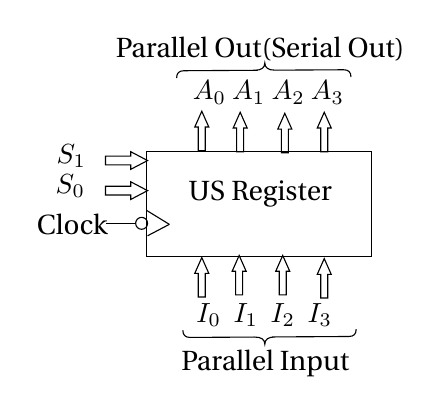
\begin{tikzpicture}[x=0.75pt,y=0.75pt,yscale=-.5,xscale=.5]
%uncomment if require: \path (0,379); %set diagram left start at 0, and has height of 379

\draw    (225.5, 113) rectangle (442.5, 214)   ;
\draw   (272,230.2) -- (278.75,215) -- (285.5,230.2) -- (282.13,230.2) -- (282.13,253) -- (275.38,253) -- (275.38,230.2) -- cycle ;
\draw   (308,228.2) -- (314.75,213) -- (321.5,228.2) -- (318.13,228.2) -- (318.13,251) -- (311.38,251) -- (311.38,228.2) -- cycle ;
\draw   (350,228.2) -- (356.75,213) -- (363.5,228.2) -- (360.13,228.2) -- (360.13,251) -- (353.38,251) -- (353.38,228.2) -- cycle ;
\draw   (390,231.2) -- (396.75,216) -- (403.5,231.2) -- (400.13,231.2) -- (400.13,254) -- (393.38,254) -- (393.38,231.2) -- cycle ;
\draw   (260.5,285) .. controls (260.53,289.67) and (262.87,291.99) .. (267.54,291.96) -- (329.46,291.59) .. controls (336.13,291.55) and (339.47,293.86) .. (339.5,298.53) .. controls (339.47,293.86) and (342.79,291.51) .. (349.46,291.47)(346.46,291.49) -- (420.54,291.05) .. controls (425.21,291.02) and (427.53,288.68) .. (427.5,284.01) ;
\draw   (272,89.2) -- (278.75,74) -- (285.5,89.2) -- (282.13,89.2) -- (282.13,112) -- (275.38,112) -- (275.38,89.2) -- cycle ;
\draw   (309,90.2) -- (315.75,75) -- (322.5,90.2) -- (319.13,90.2) -- (319.13,113) -- (312.38,113) -- (312.38,90.2) -- cycle ;
\draw   (352,91.2) -- (358.75,76) -- (365.5,91.2) -- (362.13,91.2) -- (362.13,114) -- (355.38,114) -- (355.38,91.2) -- cycle ;
\draw   (390,90.2) -- (396.75,75) -- (403.5,90.2) -- (400.13,90.2) -- (400.13,113) -- (393.38,113) -- (393.38,90.2) -- cycle ;
\draw   (422.5,41) .. controls (422.47,36.33) and (420.13,34.01) .. (415.46,34.04) -- (349.52,34.43) .. controls (342.85,34.47) and (339.51,32.16) .. (339.48,27.49) .. controls (339.51,32.16) and (336.19,34.51) .. (329.52,34.55)(332.52,34.53) -- (261.46,34.96) .. controls (256.79,34.99) and (254.47,37.33) .. (254.5,42) ;
\draw   (186,117.25) -- (210.3,117.25) -- (210.3,113) -- (226.5,121.5) -- (210.3,130) -- (210.3,125.75) -- (186,125.75) -- cycle ;
\draw   (186,146.25) -- (210.3,146.25) -- (210.3,142) -- (226.5,150.5) -- (210.3,159) -- (210.3,154.75) -- (186,154.75) -- cycle ;
\draw    (186.5,182) -- (215,182) ;


\draw    (220.75, 182) circle [x radius= 5.75, y radius= 5.75]  ;
\draw    (225.5,169.5) -- (247.5,183) ;


\draw    (247.5,183) -- (226.5,194) ;



\draw (335,14) node  [align=left] {Parallel Out(Serial Out)};
\draw (340,317) node  [align=left] {Parallel Input};
\draw (339,270) node  [align=left] {$I_0$ \  $I_1$ \  $I_2$ \  $I_3$};
\draw (343,56) node  [align=left] {$A_0$  $A_1$  $A_2$ $A_3$};
\draw (153,117) node   {$S_1$};
\draw (152,146) node   {$S_0$};
\draw (154,183) node  [align=left] {Clock};
\draw (335,154) node  [align=left] {US Register};

\end{tikzpicture}
 
\column{0.5\textwidth}
    \begin{center}
    \setbeamercovered{dynamic}
   
    \begin{tabular}{|c|c|c|}
        \hline
         $S_1$ & $S_0$ & Register Operation\\ 
        \hline \pause
        0 & 0 & No change  \\
        \hline \pause
        0 & 1 & Shift Right  \\
        \hline \pause
        1 & 0 & Shift Left    \\
        \hline \pause
        1 & 1 & Parallel Load   \\
        \hline 
    \end{tabular}
\end{center}  

\end{columns}
\end{frame}
%---------------------------------------------------------

\section{Basic Components}
\begin{frame}
\frametitle{Basic Components of Universal Shift Register}
\textbf{Universal Shift Register} has two main components -\\ 
\begin{itemize}
\item 4 to 1 Multiplexer\\ 
\item D Flip-Flop
\end{itemize}
\end{frame}

\begin{frame}
\frametitle{Components of Universal Shift Register}
\begin{itemize}
\item 4 to 1 Multiplexer\\ 
\begin{figure}[h!]
    \centering
    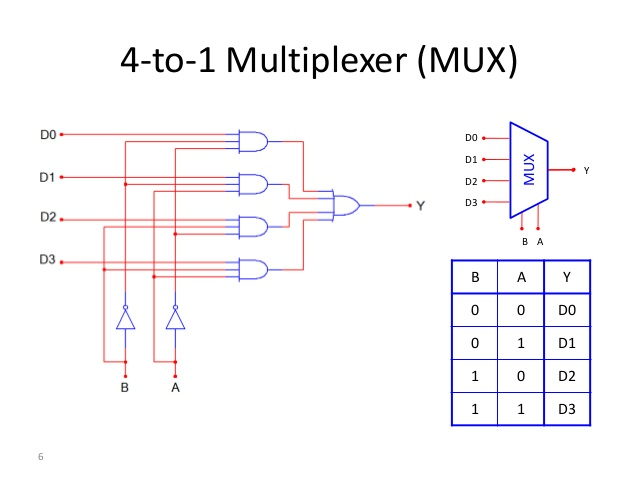
\includegraphics[width = 0.6\textwidth]{4to1mux.jpg}
\end{figure}
\end{itemize}
\end{frame}


\begin{frame}
\frametitle{Components of Universal Shift Register}
\begin{itemize}
\item D Flip-Flop\\ 
\begin{figure}[h!]
    \centering
    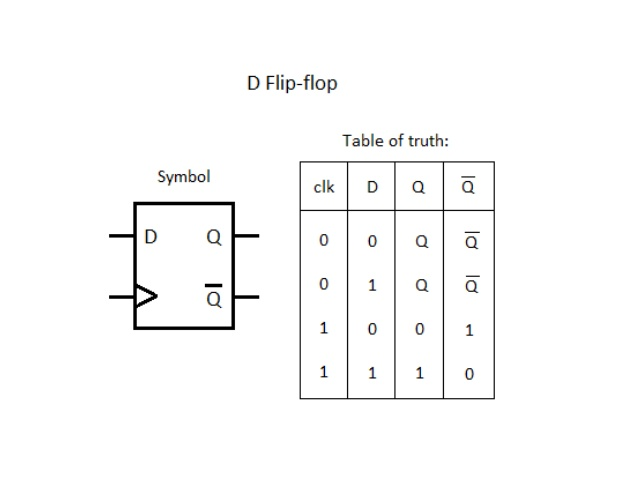
\includegraphics[width = 0.6\textwidth]{flipflop.jpg}
\end{figure}
\end{itemize}
\end{frame}

\section{Circuit Diagram}
\begin{frame}
\frametitle{Circuit Diagram}

Circuit diagram for 4 bit universal shift register  
\tikzset{every picture/.style={line width=0.75pt}} %set default line width to 0.75pt        

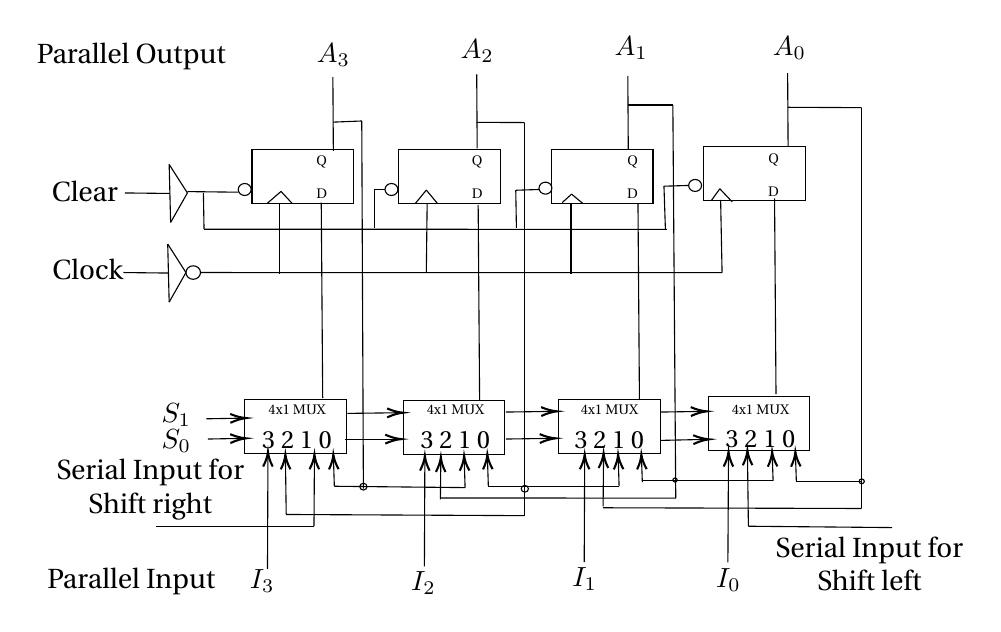
\begin{tikzpicture}[x=0.75pt,y=0.75pt,yscale=-.65,xscale=.7]
   \centering
%uncomment if require: \path (0,482.89410400390625); %set diagram left start at 0, and has height of 482.89410400390625

\draw    (247, 274) rectangle (317, 314)   ;
\draw    (138, 273) rectangle (208, 313)   ;
\draw    (354, 273) rectangle (424, 313)   ;
\draw    (457, 271) rectangle (527, 311)   ;
\draw    (244, 88) rectangle (314, 128)   ;
\draw    (143, 88) rectangle (213, 128)   ;
\draw    (349, 88) rectangle (419, 128)   ;
\draw    (454, 86) rectangle (524, 126)   ;
\draw    (111.68,287.53) -- (137,287.04) ;
\draw [shift={(139,287)}, rotate = 538.88] [color={rgb, 255:red, 0; green, 0; blue, 0 }  ][line width=0.75]    (10.93,-3.29) .. controls (6.95,-1.4) and (3.31,-0.3) .. (0,0) .. controls (3.31,0.3) and (6.95,1.4) .. (10.93,3.29)   ;

\draw    (112.68,302.53) -- (137,302.04) ;
\draw [shift={(139,302)}, rotate = 538.8399999999999] [color={rgb, 255:red, 0; green, 0; blue, 0 }  ][line width=0.75]    (10.93,-3.29) .. controls (6.95,-1.4) and (3.31,-0.3) .. (0,0) .. controls (3.31,0.3) and (6.95,1.4) .. (10.93,3.29)   ;

\draw    (153.68,398.85) -- (153.99,314) ;
\draw [shift={(154,312)}, rotate = 450.21] [color={rgb, 255:red, 0; green, 0; blue, 0 }  ][line width=0.75]    (10.93,-3.29) .. controls (6.95,-1.4) and (3.31,-0.3) .. (0,0) .. controls (3.31,0.3) and (6.95,1.4) .. (10.93,3.29)   ;

\draw    (261.68,396.85) -- (261.99,317) ;
\draw [shift={(262,315)}, rotate = 450.22] [color={rgb, 255:red, 0; green, 0; blue, 0 }  ][line width=0.75]    (10.93,-3.29) .. controls (6.95,-1.4) and (3.31,-0.3) .. (0,0) .. controls (3.31,0.3) and (6.95,1.4) .. (10.93,3.29)   ;

\draw    (371.68,393.85) -- (371.99,316) ;
\draw [shift={(372,314)}, rotate = 450.23] [color={rgb, 255:red, 0; green, 0; blue, 0 }  ][line width=0.75]    (10.93,-3.29) .. controls (6.95,-1.4) and (3.31,-0.3) .. (0,0) .. controls (3.31,0.3) and (6.95,1.4) .. (10.93,3.29)   ;

\draw    (470.56,393.89) -- (470.99,314) ;
\draw [shift={(471,312)}, rotate = 450.31] [color={rgb, 255:red, 0; green, 0; blue, 0 }  ][line width=0.75]    (10.93,-3.29) .. controls (6.95,-1.4) and (3.31,-0.3) .. (0,0) .. controls (3.31,0.3) and (6.95,1.4) .. (10.93,3.29)   ;

\draw    (185.68,367.16) -- (185.99,316) ;
\draw [shift={(186,314)}, rotate = 450.34] [color={rgb, 255:red, 0; green, 0; blue, 0 }  ][line width=0.75]    (10.93,-3.29) .. controls (6.95,-1.4) and (3.31,-0.3) .. (0,0) .. controls (3.31,0.3) and (6.95,1.4) .. (10.93,3.29)   ;

\draw    (76.68,367.16) -- (185.68,367.16) ;


\draw    (484.68,367.16) -- (484.02,313) ;
\draw [shift={(484,311)}, rotate = 449.3] [color={rgb, 255:red, 0; green, 0; blue, 0 }  ][line width=0.75]    (10.93,-3.29) .. controls (6.95,-1.4) and (3.31,-0.3) .. (0,0) .. controls (3.31,0.3) and (6.95,1.4) .. (10.93,3.29)   ;

\draw    (484.68,367.16) -- (583.68,368.16) ;


\draw    (511.68,31.27) -- (512,86) ;


\draw    (401.68,33.27) -- (402,88) ;


\draw    (297.68,32.27) -- (298,87) ;


\draw    (198.68,34.27) -- (199,89) ;


\draw    (562.68,56.9) -- (562.68,333.9) ;


\draw    (517.68,333.9) -- (562.68,333.9) ;


\draw    (511.84,56.63) -- (562.68,56.9) ;


\draw    (517.68,333.9) -- (517.06,314) ;
\draw [shift={(517,312)}, rotate = 448.21] [color={rgb, 255:red, 0; green, 0; blue, 0 }  ][line width=0.75]    (10.93,-3.29) .. controls (6.95,-1.4) and (3.31,-0.3) .. (0,0) .. controls (3.31,0.3) and (6.95,1.4) .. (10.93,3.29)   ;

\draw    (501.68,333.53) -- (501.06,314) ;
\draw [shift={(501,312)}, rotate = 448.18] [color={rgb, 255:red, 0; green, 0; blue, 0 }  ][line width=0.75]    (10.93,-3.29) .. controls (6.95,-1.4) and (3.31,-0.3) .. (0,0) .. controls (3.31,0.3) and (6.95,1.4) .. (10.93,3.29)   ;

\draw    (411.68,334.53) -- (411.07,316) ;
\draw [shift={(411,314)}, rotate = 448.09] [color={rgb, 255:red, 0; green, 0; blue, 0 }  ][line width=0.75]    (10.93,-3.29) .. controls (6.95,-1.4) and (3.31,-0.3) .. (0,0) .. controls (3.31,0.3) and (6.95,1.4) .. (10.93,3.29)   ;

\draw    (411.68,333.53) -- (501.68,333.53) ;


\draw    (562.68,354.01) -- (562.68,333.9) ;


\draw    (384.68,352.48) -- (384.98,315) ;
\draw [shift={(385,313)}, rotate = 450.46] [color={rgb, 255:red, 0; green, 0; blue, 0 }  ][line width=0.75]    (10.93,-3.29) .. controls (6.95,-1.4) and (3.31,-0.3) .. (0,0) .. controls (3.31,0.3) and (6.95,1.4) .. (10.93,3.29)   ;

\draw    (384.68,353.48) -- (562.68,354.01) ;


\draw    (305.68,337.53) -- (395.68,337.53) ;


\draw    (395.68,337.53) -- (395.06,316) ;
\draw [shift={(395,314)}, rotate = 448.33] [color={rgb, 255:red, 0; green, 0; blue, 0 }  ][line width=0.75]    (10.93,-3.29) .. controls (6.95,-1.4) and (3.31,-0.3) .. (0,0) .. controls (3.31,0.3) and (6.95,1.4) .. (10.93,3.29)   ;

\draw    (305.68,337.53) -- (305.06,316) ;
\draw [shift={(305,314)}, rotate = 448.33] [color={rgb, 255:red, 0; green, 0; blue, 0 }  ][line width=0.75]    (10.93,-3.29) .. controls (6.95,-1.4) and (3.31,-0.3) .. (0,0) .. controls (3.31,0.3) and (6.95,1.4) .. (10.93,3.29)   ;

\draw    (289.68,338.53) -- (289.06,317) ;
\draw [shift={(289,315)}, rotate = 448.33] [color={rgb, 255:red, 0; green, 0; blue, 0 }  ][line width=0.75]    (10.93,-3.29) .. controls (6.95,-1.4) and (3.31,-0.3) .. (0,0) .. controls (3.31,0.3) and (6.95,1.4) .. (10.93,3.29)   ;

\draw    (199.68,337.53) -- (199.06,316) ;
\draw [shift={(199,314)}, rotate = 448.33] [color={rgb, 255:red, 0; green, 0; blue, 0 }  ][line width=0.75]    (10.93,-3.29) .. controls (6.95,-1.4) and (3.31,-0.3) .. (0,0) .. controls (3.31,0.3) and (6.95,1.4) .. (10.93,3.29)   ;

\draw    (199.68,337.53) -- (289.68,338.53) ;


\draw    (502.68,124.22) -- (503.68,269.22) ;


\draw    (408.68,128.22) -- (409.68,273.22) ;


\draw    (298.68,129.22) -- (299.68,274.22) ;


\draw    (190.68,127.22) -- (191.68,272.22) ;


\draw    (206.68,302.59) -- (243.68,302.59) ;
\draw [shift={(245.68,302.59)}, rotate = 180] [color={rgb, 255:red, 0; green, 0; blue, 0 }  ][line width=0.75]    (10.93,-3.29) .. controls (6.95,-1.4) and (3.31,-0.3) .. (0,0) .. controls (3.31,0.3) and (6.95,1.4) .. (10.93,3.29)   ;

\draw    (317.68,302.53) -- (350,302.03) ;
\draw [shift={(352,302)}, rotate = 539.11] [color={rgb, 255:red, 0; green, 0; blue, 0 }  ][line width=0.75]    (10.93,-3.29) .. controls (6.95,-1.4) and (3.31,-0.3) .. (0,0) .. controls (3.31,0.3) and (6.95,1.4) .. (10.93,3.29)   ;

\draw    (424.68,303.53) -- (455.68,302.79) ;
\draw [shift={(457.68,302.74)}, rotate = 538.63] [color={rgb, 255:red, 0; green, 0; blue, 0 }  ][line width=0.75]    (10.93,-3.29) .. controls (6.95,-1.4) and (3.31,-0.3) .. (0,0) .. controls (3.31,0.3) and (6.95,1.4) .. (10.93,3.29)   ;

\draw    (208.68,283.53) -- (245,283.03) ;
\draw [shift={(247,283)}, rotate = 539.2] [color={rgb, 255:red, 0; green, 0; blue, 0 }  ][line width=0.75]    (10.93,-3.29) .. controls (6.95,-1.4) and (3.31,-0.3) .. (0,0) .. controls (3.31,0.3) and (6.95,1.4) .. (10.93,3.29)   ;

\draw    (317.68,282.53) -- (351,282.03) ;
\draw [shift={(353,282)}, rotate = 539.14] [color={rgb, 255:red, 0; green, 0; blue, 0 }  ][line width=0.75]    (10.93,-3.29) .. controls (6.95,-1.4) and (3.31,-0.3) .. (0,0) .. controls (3.31,0.3) and (6.95,1.4) .. (10.93,3.29)   ;

\draw    (424.68,282.53) -- (454,282.03) ;
\draw [shift={(456,282)}, rotate = 539.03] [color={rgb, 255:red, 0; green, 0; blue, 0 }  ][line width=0.75]    (10.93,-3.29) .. controls (6.95,-1.4) and (3.31,-0.3) .. (0,0) .. controls (3.31,0.3) and (6.95,1.4) .. (10.93,3.29)   ;

\draw    (272.68,347.22) -- (272.98,318) ;
\draw [shift={(273,316)}, rotate = 450.58] [color={rgb, 255:red, 0; green, 0; blue, 0 }  ][line width=0.75]    (10.93,-3.29) .. controls (6.95,-1.4) and (3.31,-0.3) .. (0,0) .. controls (3.31,0.3) and (6.95,1.4) .. (10.93,3.29)   ;

\draw    (434.68,346.32) -- (272.68,346.22) ;


\draw    (432.68,54.95) -- (434.68,346.32) ;


\draw    (401.68,54.95) -- (432.68,54.95) ;


\draw    (562.68, 333.9) circle [x radius= 1.8, y radius= 1.8]  ;
\draw    (434.18, 332.9) circle [x radius= 1.5, y radius= 1.5]  ;
\draw    (330.68,67.95) -- (330.68,359.32) ;


\draw    (166.56,358.45) -- (166.02,316) ;
\draw [shift={(166,314)}, rotate = 449.28] [color={rgb, 255:red, 0; green, 0; blue, 0 }  ][line width=0.75]    (10.93,-3.29) .. controls (6.95,-1.4) and (3.31,-0.3) .. (0,0) .. controls (3.31,0.3) and (6.95,1.4) .. (10.93,3.29)   ;

\draw    (166.56,358.45) -- (330.68,359.32) ;


\draw    (330.79, 339.39) circle [x radius= 2.5, y radius= 2.5]  ;
\draw    (297.56,67.78) -- (330.68,67.95) ;


\draw    (218.56,66.78) -- (219.68,339.32) ;


\draw    (198.84,67.63) -- (218.56,66.78) ;


\draw    (219.68, 337.84) circle [x radius= 2.5, y radius= 2.5]  ;
\draw    (55.56,120.12) -- (86.5,120.5) ;


\draw    (86,99) -- (98.56,120.12) ;


\draw    (87,142) -- (98.56,120.12) ;


\draw    (86,99) -- (87,142) ;


\draw    (138, 117.56) circle [x radius= 4.44, y radius= 4.44]  ;
\draw    (239, 117.56) circle [x radius= 4.44, y radius= 4.44]  ;
\draw    (345, 116.56) circle [x radius= 4.44, y radius= 4.44]  ;
\draw    (448, 114.56) circle [x radius= 4.44, y radius= 4.44]  ;
\draw    (98.56,119.12) -- (133.56,119.56) ;


\draw    (110,147) -- (428.56,147.12) ;


\draw    (110,147) -- (109.56,120.12) ;


\draw    (227.56,117.56) -- (227.56,146.12) ;


\draw    (227.56,117.56) -- (234.56,117.56) ;


\draw    (325,146) -- (324.56,118.12) ;


\draw    (324.56,118.12) -- (340.56,117.56) ;


\draw    (427.56,147.12) -- (426.56,115.12) ;


\draw    (426.56,115.12) -- (443.56,114.56) ;


\draw    (54.56,179.12) -- (85.5,179.5) ;


\draw    (85,158) -- (97.56,179.12) ;


\draw    (86,201) -- (97.56,179.12) ;


\draw    (85,158) -- (86,201) ;


\draw    (107.56,179.12) -- (466.56,179.23) ;


\draw    (102.56, 179.12) circle [x radius= 5, y radius= 5]  ;
\draw    (465.56,125.23) -- (466.56,179.23) ;


\draw    (362.56,127.23) -- (362.56,180.23) ;


\draw    (263.56,128.23) -- (263,179) ;


\draw    (162,128) -- (162,180) ;


\draw    (163,119) -- (170.56,127.78) ;


\draw    (163,119) -- (153.56,127.78) ;


\draw    (263,118) -- (270.56,127.78) ;


\draw    (263,118) -- (255.56,127.78) ;


\draw    (363,121) -- (370.56,127.78) ;


\draw    (363,121) -- (356.56,127.23) ;


\draw    (465,117) -- (473.56,126.78) ;


\draw    (465,117) -- (459,126) ;



\draw (150,408) node  [align=center] {$I_3$};
\draw (261,409) node  [align=center] {$I_2$};
\draw (372,406) node [align=center]{$I_1$};
\draw (471,407) node [align=center] {$I_0$};
\draw (73,340) node  [align=center] {Serial Input for\\Shift right};
\draw (568,395) node  [align=center] {Serial Input for\\Shift left};
\draw (91,285) node  [align=center] {$S_1$};
\draw (91,304) node [align=center] {$S_0$};
\draw (199,18) node  [align=center] {$A_3$};
\draw (298,15) node  [align=center] {$A_2$};
\draw (404,13) node  [align=center] {$A_1$};
\draw (513,13) node  [align=center] {$A_0$};
\draw (60,408) node  [align=center] {Parallel Input};
\draw (60,19) node  [align=center] {Parallel Output};
\draw (28,119) node  [align=center] {Clear};
\draw (30,177) node  [align=center] {Clock};
\draw (191,108.5) node  [align=center] {\tiny Q\\\tiny D};
\draw (298,108.5) node  [align=center] {\tiny Q\\\tiny D};
\draw (405,108.5) node  [align=center] {\tiny Q\\\tiny D};
\draw (502,107) node  [align=center] {\tiny Q\\\tiny D};
\draw (174,293.5) node [align=center] {\tiny 4x1 MUX\\\small 3 2 1 0};
\draw (283,293.5) node  [align=center] {\tiny 4x1 MUX\\\small 3 2 1 0};
\draw (389,293.5) node  [align=center] {\tiny 4x1 MUX\\\small 3 2 1 0};
\draw (493,293) node  [align=center] {\tiny 4x1 MUX\\\small 3 2 1 0};


\end{tikzpicture}
\end{frame}
\begin{frame}
\frametitle{Unchanged of Output in Universal Shift Register}
When $S_0=0$ and $S_1=0$,output will changed.
\tikzset{every picture/.style={line width=0.75pt}} %set default line width to 0.75pt        

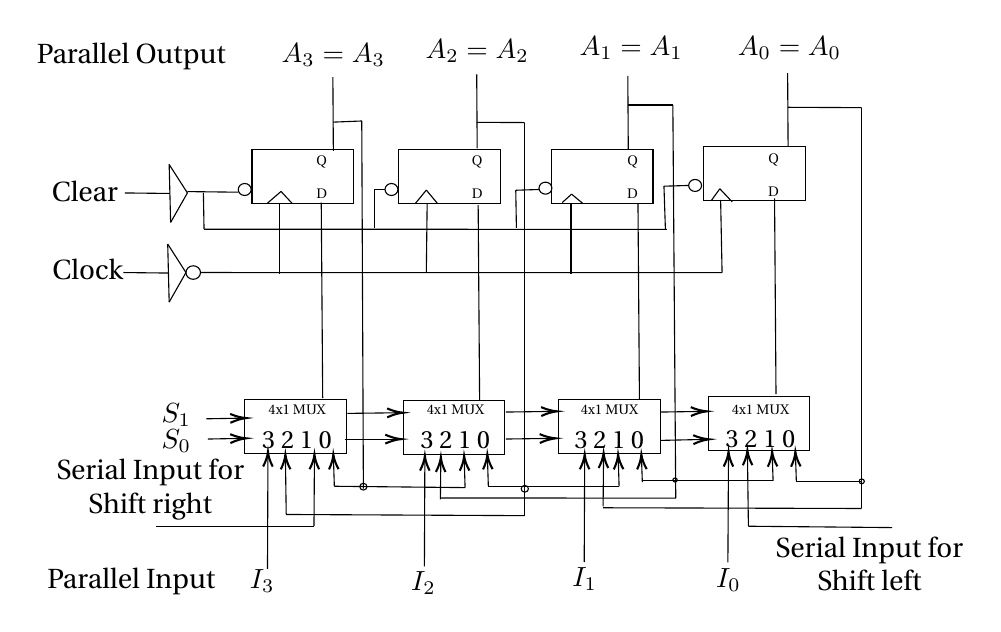
\begin{tikzpicture}[x=0.75pt,y=0.75pt,yscale=-.65,xscale=.7]
   \centering
%uncomment if require: \path (0,482.89410400390625); %set diagram left start at 0, and has height of 482.89410400390625

\draw    (247, 274) rectangle (317, 314)   ;
\draw    (138, 273) rectangle (208, 313)   ;
\draw    (354, 273) rectangle (424, 313)   ;
\draw    (457, 271) rectangle (527, 311)   ;
\draw    (244, 88) rectangle (314, 128)   ;
\draw    (143, 88) rectangle (213, 128)   ;
\draw    (349, 88) rectangle (419, 128)   ;
\draw    (454, 86) rectangle (524, 126)   ;
\draw    (111.68,287.53) -- (137,287.04) ;
\draw [shift={(139,287)}, rotate = 538.88] [color={rgb, 255:red, 0; green, 0; blue, 0 }  ][line width=0.75]    (10.93,-3.29) .. controls (6.95,-1.4) and (3.31,-0.3) .. (0,0) .. controls (3.31,0.3) and (6.95,1.4) .. (10.93,3.29)   ;

\draw    (112.68,302.53) -- (137,302.04) ;
\draw [shift={(139,302)}, rotate = 538.8399999999999] [color={rgb, 255:red, 0; green, 0; blue, 0 }  ][line width=0.75]    (10.93,-3.29) .. controls (6.95,-1.4) and (3.31,-0.3) .. (0,0) .. controls (3.31,0.3) and (6.95,1.4) .. (10.93,3.29)   ;

\draw    (153.68,398.85) -- (153.99,314) ;
\draw [shift={(154,312)}, rotate = 450.21] [color={rgb, 255:red, 0; green, 0; blue, 0 }  ][line width=0.75]    (10.93,-3.29) .. controls (6.95,-1.4) and (3.31,-0.3) .. (0,0) .. controls (3.31,0.3) and (6.95,1.4) .. (10.93,3.29)   ;

\draw    (261.68,396.85) -- (261.99,317) ;
\draw [shift={(262,315)}, rotate = 450.22] [color={rgb, 255:red, 0; green, 0; blue, 0 }  ][line width=0.75]    (10.93,-3.29) .. controls (6.95,-1.4) and (3.31,-0.3) .. (0,0) .. controls (3.31,0.3) and (6.95,1.4) .. (10.93,3.29)   ;

\draw    (371.68,393.85) -- (371.99,316) ;
\draw [shift={(372,314)}, rotate = 450.23] [color={rgb, 255:red, 0; green, 0; blue, 0 }  ][line width=0.75]    (10.93,-3.29) .. controls (6.95,-1.4) and (3.31,-0.3) .. (0,0) .. controls (3.31,0.3) and (6.95,1.4) .. (10.93,3.29)   ;

\draw    (470.56,393.89) -- (470.99,314) ;
\draw [shift={(471,312)}, rotate = 450.31] [color={rgb, 255:red, 0; green, 0; blue, 0 }  ][line width=0.75]    (10.93,-3.29) .. controls (6.95,-1.4) and (3.31,-0.3) .. (0,0) .. controls (3.31,0.3) and (6.95,1.4) .. (10.93,3.29)   ;

\draw    (185.68,367.16) -- (185.99,316) ;
\draw [shift={(186,314)}, rotate = 450.34] [color={rgb, 255:red, 0; green, 0; blue, 0 }  ][line width=0.75]    (10.93,-3.29) .. controls (6.95,-1.4) and (3.31,-0.3) .. (0,0) .. controls (3.31,0.3) and (6.95,1.4) .. (10.93,3.29)   ;

\draw    (76.68,367.16) -- (185.68,367.16) ;


\draw    (484.68,367.16) -- (484.02,313) ;
\draw [shift={(484,311)}, rotate = 449.3] [color={rgb, 255:red, 0; green, 0; blue, 0 }  ][line width=0.75]    (10.93,-3.29) .. controls (6.95,-1.4) and (3.31,-0.3) .. (0,0) .. controls (3.31,0.3) and (6.95,1.4) .. (10.93,3.29)   ;

\draw    (484.68,367.16) -- (583.68,368.16) ;


\draw    (511.68,31.27) -- (512,86) ;


\draw    (401.68,33.27) -- (402,88) ;


\draw    (297.68,32.27) -- (298,87) ;


\draw    (198.68,34.27) -- (199,89) ;


\draw    (562.68,56.9) -- (562.68,333.9) ;


\draw    (517.68,333.9) -- (562.68,333.9) ;


\draw    (511.84,56.63) -- (562.68,56.9) ;


\draw    (517.68,333.9) -- (517.06,314) ;
\draw [shift={(517,312)}, rotate = 448.21] [color={rgb, 255:red, 0; green, 0; blue, 0 }  ][line width=0.75]    (10.93,-3.29) .. controls (6.95,-1.4) and (3.31,-0.3) .. (0,0) .. controls (3.31,0.3) and (6.95,1.4) .. (10.93,3.29)   ;

\draw    (501.68,333.53) -- (501.06,314) ;
\draw [shift={(501,312)}, rotate = 448.18] [color={rgb, 255:red, 0; green, 0; blue, 0 }  ][line width=0.75]    (10.93,-3.29) .. controls (6.95,-1.4) and (3.31,-0.3) .. (0,0) .. controls (3.31,0.3) and (6.95,1.4) .. (10.93,3.29)   ;

\draw    (411.68,334.53) -- (411.07,316) ;
\draw [shift={(411,314)}, rotate = 448.09] [color={rgb, 255:red, 0; green, 0; blue, 0 }  ][line width=0.75]    (10.93,-3.29) .. controls (6.95,-1.4) and (3.31,-0.3) .. (0,0) .. controls (3.31,0.3) and (6.95,1.4) .. (10.93,3.29)   ;

\draw    (411.68,333.53) -- (501.68,333.53) ;


\draw    (562.68,354.01) -- (562.68,333.9) ;


\draw    (384.68,352.48) -- (384.98,315) ;
\draw [shift={(385,313)}, rotate = 450.46] [color={rgb, 255:red, 0; green, 0; blue, 0 }  ][line width=0.75]    (10.93,-3.29) .. controls (6.95,-1.4) and (3.31,-0.3) .. (0,0) .. controls (3.31,0.3) and (6.95,1.4) .. (10.93,3.29)   ;

\draw    (384.68,353.48) -- (562.68,354.01) ;


\draw    (305.68,337.53) -- (395.68,337.53) ;


\draw    (395.68,337.53) -- (395.06,316) ;
\draw [shift={(395,314)}, rotate = 448.33] [color={rgb, 255:red, 0; green, 0; blue, 0 }  ][line width=0.75]    (10.93,-3.29) .. controls (6.95,-1.4) and (3.31,-0.3) .. (0,0) .. controls (3.31,0.3) and (6.95,1.4) .. (10.93,3.29)   ;

\draw    (305.68,337.53) -- (305.06,316) ;
\draw [shift={(305,314)}, rotate = 448.33] [color={rgb, 255:red, 0; green, 0; blue, 0 }  ][line width=0.75]    (10.93,-3.29) .. controls (6.95,-1.4) and (3.31,-0.3) .. (0,0) .. controls (3.31,0.3) and (6.95,1.4) .. (10.93,3.29)   ;

\draw    (289.68,338.53) -- (289.06,317) ;
\draw [shift={(289,315)}, rotate = 448.33] [color={rgb, 255:red, 0; green, 0; blue, 0 }  ][line width=0.75]    (10.93,-3.29) .. controls (6.95,-1.4) and (3.31,-0.3) .. (0,0) .. controls (3.31,0.3) and (6.95,1.4) .. (10.93,3.29)   ;

\draw    (199.68,337.53) -- (199.06,316) ;
\draw [shift={(199,314)}, rotate = 448.33] [color={rgb, 255:red, 0; green, 0; blue, 0 }  ][line width=0.75]    (10.93,-3.29) .. controls (6.95,-1.4) and (3.31,-0.3) .. (0,0) .. controls (3.31,0.3) and (6.95,1.4) .. (10.93,3.29)   ;

\draw    (199.68,337.53) -- (289.68,338.53) ;


\draw    (502.68,124.22) -- (503.68,269.22) ;


\draw    (408.68,128.22) -- (409.68,273.22) ;


\draw    (298.68,129.22) -- (299.68,274.22) ;


\draw    (190.68,127.22) -- (191.68,272.22) ;


\draw    (206.68,302.59) -- (243.68,302.59) ;
\draw [shift={(245.68,302.59)}, rotate = 180] [color={rgb, 255:red, 0; green, 0; blue, 0 }  ][line width=0.75]    (10.93,-3.29) .. controls (6.95,-1.4) and (3.31,-0.3) .. (0,0) .. controls (3.31,0.3) and (6.95,1.4) .. (10.93,3.29)   ;

\draw    (317.68,302.53) -- (350,302.03) ;
\draw [shift={(352,302)}, rotate = 539.11] [color={rgb, 255:red, 0; green, 0; blue, 0 }  ][line width=0.75]    (10.93,-3.29) .. controls (6.95,-1.4) and (3.31,-0.3) .. (0,0) .. controls (3.31,0.3) and (6.95,1.4) .. (10.93,3.29)   ;

\draw    (424.68,303.53) -- (455.68,302.79) ;
\draw [shift={(457.68,302.74)}, rotate = 538.63] [color={rgb, 255:red, 0; green, 0; blue, 0 }  ][line width=0.75]    (10.93,-3.29) .. controls (6.95,-1.4) and (3.31,-0.3) .. (0,0) .. controls (3.31,0.3) and (6.95,1.4) .. (10.93,3.29)   ;

\draw    (208.68,283.53) -- (245,283.03) ;
\draw [shift={(247,283)}, rotate = 539.2] [color={rgb, 255:red, 0; green, 0; blue, 0 }  ][line width=0.75]    (10.93,-3.29) .. controls (6.95,-1.4) and (3.31,-0.3) .. (0,0) .. controls (3.31,0.3) and (6.95,1.4) .. (10.93,3.29)   ;

\draw    (317.68,282.53) -- (351,282.03) ;
\draw [shift={(353,282)}, rotate = 539.14] [color={rgb, 255:red, 0; green, 0; blue, 0 }  ][line width=0.75]    (10.93,-3.29) .. controls (6.95,-1.4) and (3.31,-0.3) .. (0,0) .. controls (3.31,0.3) and (6.95,1.4) .. (10.93,3.29)   ;

\draw    (424.68,282.53) -- (454,282.03) ;
\draw [shift={(456,282)}, rotate = 539.03] [color={rgb, 255:red, 0; green, 0; blue, 0 }  ][line width=0.75]    (10.93,-3.29) .. controls (6.95,-1.4) and (3.31,-0.3) .. (0,0) .. controls (3.31,0.3) and (6.95,1.4) .. (10.93,3.29)   ;

\draw    (272.68,347.22) -- (272.98,318) ;
\draw [shift={(273,316)}, rotate = 450.58] [color={rgb, 255:red, 0; green, 0; blue, 0 }  ][line width=0.75]    (10.93,-3.29) .. controls (6.95,-1.4) and (3.31,-0.3) .. (0,0) .. controls (3.31,0.3) and (6.95,1.4) .. (10.93,3.29)   ;

\draw    (434.68,346.32) -- (272.68,346.22) ;


\draw    (432.68,54.95) -- (434.68,346.32) ;


\draw    (401.68,54.95) -- (432.68,54.95) ;


\draw    (562.68, 333.9) circle [x radius= 1.8, y radius= 1.8]  ;
\draw    (434.18, 332.9) circle [x radius= 1.5, y radius= 1.5]  ;
\draw    (330.68,67.95) -- (330.68,359.32) ;


\draw    (166.56,358.45) -- (166.02,316) ;
\draw [shift={(166,314)}, rotate = 449.28] [color={rgb, 255:red, 0; green, 0; blue, 0 }  ][line width=0.75]    (10.93,-3.29) .. controls (6.95,-1.4) and (3.31,-0.3) .. (0,0) .. controls (3.31,0.3) and (6.95,1.4) .. (10.93,3.29)   ;

\draw    (166.56,358.45) -- (330.68,359.32) ;


\draw    (330.79, 339.39) circle [x radius= 2.5, y radius= 2.5]  ;
\draw    (297.56,67.78) -- (330.68,67.95) ;


\draw    (218.56,66.78) -- (219.68,339.32) ;


\draw    (198.84,67.63) -- (218.56,66.78) ;


\draw    (219.68, 337.84) circle [x radius= 2.5, y radius= 2.5]  ;
\draw    (55.56,120.12) -- (86.5,120.5) ;


\draw    (86,99) -- (98.56,120.12) ;


\draw    (87,142) -- (98.56,120.12) ;


\draw    (86,99) -- (87,142) ;


\draw    (138, 117.56) circle [x radius= 4.44, y radius= 4.44]  ;
\draw    (239, 117.56) circle [x radius= 4.44, y radius= 4.44]  ;
\draw    (345, 116.56) circle [x radius= 4.44, y radius= 4.44]  ;
\draw    (448, 114.56) circle [x radius= 4.44, y radius= 4.44]  ;
\draw    (98.56,119.12) -- (133.56,119.56) ;


\draw    (110,147) -- (428.56,147.12) ;


\draw    (110,147) -- (109.56,120.12) ;


\draw    (227.56,117.56) -- (227.56,146.12) ;


\draw    (227.56,117.56) -- (234.56,117.56) ;


\draw    (325,146) -- (324.56,118.12) ;


\draw    (324.56,118.12) -- (340.56,117.56) ;


\draw    (427.56,147.12) -- (426.56,115.12) ;


\draw    (426.56,115.12) -- (443.56,114.56) ;


\draw    (54.56,179.12) -- (85.5,179.5) ;


\draw    (85,158) -- (97.56,179.12) ;


\draw    (86,201) -- (97.56,179.12) ;


\draw    (85,158) -- (86,201) ;


\draw    (107.56,179.12) -- (466.56,179.23) ;


\draw    (102.56, 179.12) circle [x radius= 5, y radius= 5]  ;
\draw    (465.56,125.23) -- (466.56,179.23) ;


\draw    (362.56,127.23) -- (362.56,180.23) ;


\draw    (263.56,128.23) -- (263,179) ;


\draw    (162,128) -- (162,180) ;


\draw    (163,119) -- (170.56,127.78) ;


\draw    (163,119) -- (153.56,127.78) ;


\draw    (263,118) -- (270.56,127.78) ;


\draw    (263,118) -- (255.56,127.78) ;


\draw    (363,121) -- (370.56,127.78) ;


\draw    (363,121) -- (356.56,127.23) ;


\draw    (465,117) -- (473.56,126.78) ;


\draw    (465,117) -- (459,126) ;



\draw (150,408) node  [align=center] {$I_3$};
\draw (261,409) node  [align=center] {$I_2$};
\draw (372,406) node [align=center]{$I_1$};
\draw (471,407) node [align=center] {$I_0$};
\draw (73,340) node  [align=center] {Serial Input for\\Shift right};
\draw (568,395) node  [align=center] {Serial Input for\\Shift left};
\draw (91,285) node  [align=center] {$S_1$};
\draw (91,304) node [align=center] {$S_0$};
\draw (199,18) node  [align=center] {$A_3=A_3$};
\draw (298,15) node  [align=center] {$A_2=A_2$};
\draw (404,13) node  [align=center] {$A_1=A_1$};
\draw (513,13) node  [align=center] {$A_0=A_0$};
\draw (60,408) node  [align=center] {Parallel Input};
\draw (60,19) node  [align=center] {Parallel Output};
\draw (28,119) node  [align=center] {Clear};
\draw (30,177) node  [align=center] {Clock};
\draw (191,108.5) node  [align=center] {\tiny Q\\\tiny D};
\draw (298,108.5) node  [align=center] {\tiny Q\\\tiny D};
\draw (405,108.5) node  [align=center] {\tiny Q\\\tiny D};
\draw (502,107) node  [align=center] {\tiny Q\\\tiny D};
\draw (174,293.5) node [align=center] {\tiny 4x1 MUX\\\small 3 2 1 0};
\draw (283,293.5) node  [align=center] {\tiny 4x1 MUX\\\small 3 2 1 0};
\draw (389,293.5) node  [align=center] {\tiny 4x1 MUX\\\small 3 2 1 0};
\draw (493,293) node  [align=center] {\tiny 4x1 MUX\\\small 3 2 1 0};


\end{tikzpicture}
\end{frame}
\begin{frame}
\frametitle{Right Shift in Universal Shift Register}
When $S_0=1$ and $S_1=0$,data will be shifted right.
\tikzset{every picture/.style={line width=0.75pt}} %set default line width to 0.75pt        

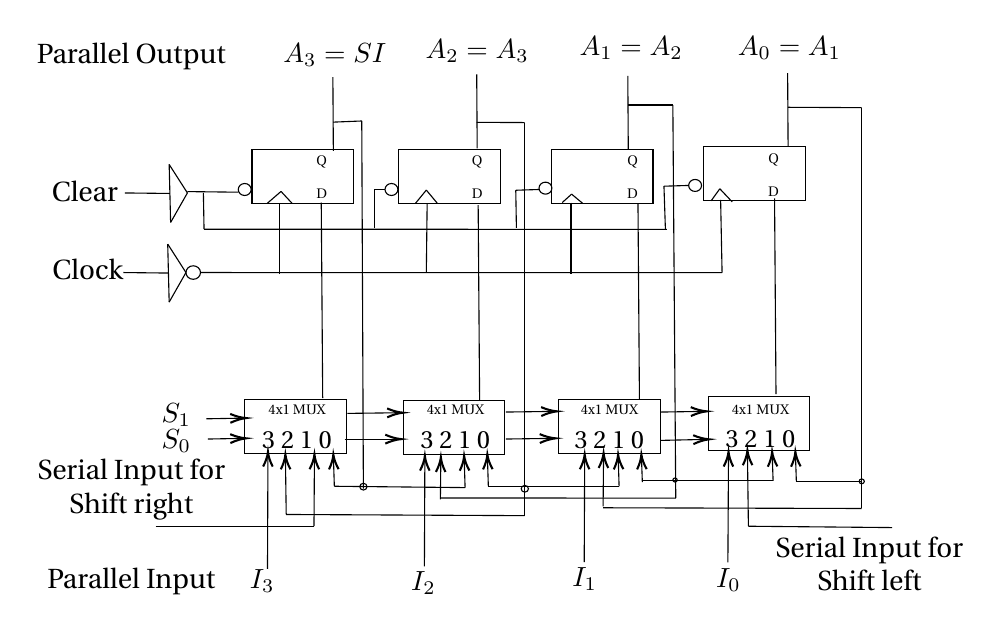
\begin{tikzpicture}[x=0.75pt,y=0.75pt,yscale=-.65,xscale=.7]
   \centering
%uncomment if require: \path (0,482.89410400390625); %set diagram left start at 0, and has height of 482.89410400390625

\draw    (247, 274) rectangle (317, 314)   ;
\draw    (138, 273) rectangle (208, 313)   ;
\draw    (354, 273) rectangle (424, 313)   ;
\draw    (457, 271) rectangle (527, 311)   ;
\draw    (244, 88) rectangle (314, 128)   ;
\draw    (143, 88) rectangle (213, 128)   ;
\draw    (349, 88) rectangle (419, 128)   ;
\draw    (454, 86) rectangle (524, 126)   ;
\draw    (111.68,287.53) -- (137,287.04) ;
\draw [shift={(139,287)}, rotate = 538.88] [color={rgb, 255:red, 0; green, 0; blue, 0 }  ][line width=0.75]    (10.93,-3.29) .. controls (6.95,-1.4) and (3.31,-0.3) .. (0,0) .. controls (3.31,0.3) and (6.95,1.4) .. (10.93,3.29)   ;

\draw    (112.68,302.53) -- (137,302.04) ;
\draw [shift={(139,302)}, rotate = 538.8399999999999] [color={rgb, 255:red, 0; green, 0; blue, 0 }  ][line width=0.75]    (10.93,-3.29) .. controls (6.95,-1.4) and (3.31,-0.3) .. (0,0) .. controls (3.31,0.3) and (6.95,1.4) .. (10.93,3.29)   ;

\draw    (153.68,398.85) -- (153.99,314) ;
\draw [shift={(154,312)}, rotate = 450.21] [color={rgb, 255:red, 0; green, 0; blue, 0 }  ][line width=0.75]    (10.93,-3.29) .. controls (6.95,-1.4) and (3.31,-0.3) .. (0,0) .. controls (3.31,0.3) and (6.95,1.4) .. (10.93,3.29)   ;

\draw    (261.68,396.85) -- (261.99,317) ;
\draw [shift={(262,315)}, rotate = 450.22] [color={rgb, 255:red, 0; green, 0; blue, 0 }  ][line width=0.75]    (10.93,-3.29) .. controls (6.95,-1.4) and (3.31,-0.3) .. (0,0) .. controls (3.31,0.3) and (6.95,1.4) .. (10.93,3.29)   ;

\draw    (371.68,393.85) -- (371.99,316) ;
\draw [shift={(372,314)}, rotate = 450.23] [color={rgb, 255:red, 0; green, 0; blue, 0 }  ][line width=0.75]    (10.93,-3.29) .. controls (6.95,-1.4) and (3.31,-0.3) .. (0,0) .. controls (3.31,0.3) and (6.95,1.4) .. (10.93,3.29)   ;

\draw    (470.56,393.89) -- (470.99,314) ;
\draw [shift={(471,312)}, rotate = 450.31] [color={rgb, 255:red, 0; green, 0; blue, 0 }  ][line width=0.75]    (10.93,-3.29) .. controls (6.95,-1.4) and (3.31,-0.3) .. (0,0) .. controls (3.31,0.3) and (6.95,1.4) .. (10.93,3.29)   ;

\draw    (185.68,367.16) -- (185.99,316) ;
\draw [shift={(186,314)}, rotate = 450.34] [color={rgb, 255:red, 0; green, 0; blue, 0 }  ][line width=0.75]    (10.93,-3.29) .. controls (6.95,-1.4) and (3.31,-0.3) .. (0,0) .. controls (3.31,0.3) and (6.95,1.4) .. (10.93,3.29)   ;

\draw    (76.68,367.16) -- (185.68,367.16) ;


\draw    (484.68,367.16) -- (484.02,313) ;
\draw [shift={(484,311)}, rotate = 449.3] [color={rgb, 255:red, 0; green, 0; blue, 0 }  ][line width=0.75]    (10.93,-3.29) .. controls (6.95,-1.4) and (3.31,-0.3) .. (0,0) .. controls (3.31,0.3) and (6.95,1.4) .. (10.93,3.29)   ;

\draw    (484.68,367.16) -- (583.68,368.16) ;


\draw    (511.68,31.27) -- (512,86) ;


\draw    (401.68,33.27) -- (402,88) ;


\draw    (297.68,32.27) -- (298,87) ;


\draw    (198.68,34.27) -- (199,89) ;


\draw    (562.68,56.9) -- (562.68,333.9) ;


\draw    (517.68,333.9) -- (562.68,333.9) ;


\draw    (511.84,56.63) -- (562.68,56.9) ;


\draw    (517.68,333.9) -- (517.06,314) ;
\draw [shift={(517,312)}, rotate = 448.21] [color={rgb, 255:red, 0; green, 0; blue, 0 }  ][line width=0.75]    (10.93,-3.29) .. controls (6.95,-1.4) and (3.31,-0.3) .. (0,0) .. controls (3.31,0.3) and (6.95,1.4) .. (10.93,3.29)   ;

\draw    (501.68,333.53) -- (501.06,314) ;
\draw [shift={(501,312)}, rotate = 448.18] [color={rgb, 255:red, 0; green, 0; blue, 0 }  ][line width=0.75]    (10.93,-3.29) .. controls (6.95,-1.4) and (3.31,-0.3) .. (0,0) .. controls (3.31,0.3) and (6.95,1.4) .. (10.93,3.29)   ;

\draw    (411.68,334.53) -- (411.07,316) ;
\draw [shift={(411,314)}, rotate = 448.09] [color={rgb, 255:red, 0; green, 0; blue, 0 }  ][line width=0.75]    (10.93,-3.29) .. controls (6.95,-1.4) and (3.31,-0.3) .. (0,0) .. controls (3.31,0.3) and (6.95,1.4) .. (10.93,3.29)   ;

\draw    (411.68,333.53) -- (501.68,333.53) ;


\draw    (562.68,354.01) -- (562.68,333.9) ;


\draw    (384.68,352.48) -- (384.98,315) ;
\draw [shift={(385,313)}, rotate = 450.46] [color={rgb, 255:red, 0; green, 0; blue, 0 }  ][line width=0.75]    (10.93,-3.29) .. controls (6.95,-1.4) and (3.31,-0.3) .. (0,0) .. controls (3.31,0.3) and (6.95,1.4) .. (10.93,3.29)   ;

\draw    (384.68,353.48) -- (562.68,354.01) ;


\draw    (305.68,337.53) -- (395.68,337.53) ;


\draw    (395.68,337.53) -- (395.06,316) ;
\draw [shift={(395,314)}, rotate = 448.33] [color={rgb, 255:red, 0; green, 0; blue, 0 }  ][line width=0.75]    (10.93,-3.29) .. controls (6.95,-1.4) and (3.31,-0.3) .. (0,0) .. controls (3.31,0.3) and (6.95,1.4) .. (10.93,3.29)   ;

\draw    (305.68,337.53) -- (305.06,316) ;
\draw [shift={(305,314)}, rotate = 448.33] [color={rgb, 255:red, 0; green, 0; blue, 0 }  ][line width=0.75]    (10.93,-3.29) .. controls (6.95,-1.4) and (3.31,-0.3) .. (0,0) .. controls (3.31,0.3) and (6.95,1.4) .. (10.93,3.29)   ;

\draw    (289.68,338.53) -- (289.06,317) ;
\draw [shift={(289,315)}, rotate = 448.33] [color={rgb, 255:red, 0; green, 0; blue, 0 }  ][line width=0.75]    (10.93,-3.29) .. controls (6.95,-1.4) and (3.31,-0.3) .. (0,0) .. controls (3.31,0.3) and (6.95,1.4) .. (10.93,3.29)   ;

\draw    (199.68,337.53) -- (199.06,316) ;
\draw [shift={(199,314)}, rotate = 448.33] [color={rgb, 255:red, 0; green, 0; blue, 0 }  ][line width=0.75]    (10.93,-3.29) .. controls (6.95,-1.4) and (3.31,-0.3) .. (0,0) .. controls (3.31,0.3) and (6.95,1.4) .. (10.93,3.29)   ;

\draw    (199.68,337.53) -- (289.68,338.53) ;


\draw    (502.68,124.22) -- (503.68,269.22) ;


\draw    (408.68,128.22) -- (409.68,273.22) ;


\draw    (298.68,129.22) -- (299.68,274.22) ;


\draw    (190.68,127.22) -- (191.68,272.22) ;


\draw    (206.68,302.59) -- (243.68,302.59) ;
\draw [shift={(245.68,302.59)}, rotate = 180] [color={rgb, 255:red, 0; green, 0; blue, 0 }  ][line width=0.75]    (10.93,-3.29) .. controls (6.95,-1.4) and (3.31,-0.3) .. (0,0) .. controls (3.31,0.3) and (6.95,1.4) .. (10.93,3.29)   ;

\draw    (317.68,302.53) -- (350,302.03) ;
\draw [shift={(352,302)}, rotate = 539.11] [color={rgb, 255:red, 0; green, 0; blue, 0 }  ][line width=0.75]    (10.93,-3.29) .. controls (6.95,-1.4) and (3.31,-0.3) .. (0,0) .. controls (3.31,0.3) and (6.95,1.4) .. (10.93,3.29)   ;

\draw    (424.68,303.53) -- (455.68,302.79) ;
\draw [shift={(457.68,302.74)}, rotate = 538.63] [color={rgb, 255:red, 0; green, 0; blue, 0 }  ][line width=0.75]    (10.93,-3.29) .. controls (6.95,-1.4) and (3.31,-0.3) .. (0,0) .. controls (3.31,0.3) and (6.95,1.4) .. (10.93,3.29)   ;

\draw    (208.68,283.53) -- (245,283.03) ;
\draw [shift={(247,283)}, rotate = 539.2] [color={rgb, 255:red, 0; green, 0; blue, 0 }  ][line width=0.75]    (10.93,-3.29) .. controls (6.95,-1.4) and (3.31,-0.3) .. (0,0) .. controls (3.31,0.3) and (6.95,1.4) .. (10.93,3.29)   ;

\draw    (317.68,282.53) -- (351,282.03) ;
\draw [shift={(353,282)}, rotate = 539.14] [color={rgb, 255:red, 0; green, 0; blue, 0 }  ][line width=0.75]    (10.93,-3.29) .. controls (6.95,-1.4) and (3.31,-0.3) .. (0,0) .. controls (3.31,0.3) and (6.95,1.4) .. (10.93,3.29)   ;

\draw    (424.68,282.53) -- (454,282.03) ;
\draw [shift={(456,282)}, rotate = 539.03] [color={rgb, 255:red, 0; green, 0; blue, 0 }  ][line width=0.75]    (10.93,-3.29) .. controls (6.95,-1.4) and (3.31,-0.3) .. (0,0) .. controls (3.31,0.3) and (6.95,1.4) .. (10.93,3.29)   ;

\draw    (272.68,347.22) -- (272.98,318) ;
\draw [shift={(273,316)}, rotate = 450.58] [color={rgb, 255:red, 0; green, 0; blue, 0 }  ][line width=0.75]    (10.93,-3.29) .. controls (6.95,-1.4) and (3.31,-0.3) .. (0,0) .. controls (3.31,0.3) and (6.95,1.4) .. (10.93,3.29)   ;

\draw    (434.68,346.32) -- (272.68,346.22) ;


\draw    (432.68,54.95) -- (434.68,346.32) ;


\draw    (401.68,54.95) -- (432.68,54.95) ;


\draw    (562.68, 333.9) circle [x radius= 1.8, y radius= 1.8]  ;
\draw    (434.18, 332.9) circle [x radius= 1.5, y radius= 1.5]  ;
\draw    (330.68,67.95) -- (330.68,359.32) ;


\draw    (166.56,358.45) -- (166.02,316) ;
\draw [shift={(166,314)}, rotate = 449.28] [color={rgb, 255:red, 0; green, 0; blue, 0 }  ][line width=0.75]    (10.93,-3.29) .. controls (6.95,-1.4) and (3.31,-0.3) .. (0,0) .. controls (3.31,0.3) and (6.95,1.4) .. (10.93,3.29)   ;

\draw    (166.56,358.45) -- (330.68,359.32) ;


\draw    (330.79, 339.39) circle [x radius= 2.5, y radius= 2.5]  ;
\draw    (297.56,67.78) -- (330.68,67.95) ;


\draw    (218.56,66.78) -- (219.68,339.32) ;


\draw    (198.84,67.63) -- (218.56,66.78) ;


\draw    (219.68, 337.84) circle [x radius= 2.5, y radius= 2.5]  ;
\draw    (55.56,120.12) -- (86.5,120.5) ;


\draw    (86,99) -- (98.56,120.12) ;


\draw    (87,142) -- (98.56,120.12) ;


\draw    (86,99) -- (87,142) ;


\draw    (138, 117.56) circle [x radius= 4.44, y radius= 4.44]  ;
\draw    (239, 117.56) circle [x radius= 4.44, y radius= 4.44]  ;
\draw    (345, 116.56) circle [x radius= 4.44, y radius= 4.44]  ;
\draw    (448, 114.56) circle [x radius= 4.44, y radius= 4.44]  ;
\draw    (98.56,119.12) -- (133.56,119.56) ;


\draw    (110,147) -- (428.56,147.12) ;


\draw    (110,147) -- (109.56,120.12) ;


\draw    (227.56,117.56) -- (227.56,146.12) ;


\draw    (227.56,117.56) -- (234.56,117.56) ;


\draw    (325,146) -- (324.56,118.12) ;


\draw    (324.56,118.12) -- (340.56,117.56) ;


\draw    (427.56,147.12) -- (426.56,115.12) ;


\draw    (426.56,115.12) -- (443.56,114.56) ;


\draw    (54.56,179.12) -- (85.5,179.5) ;


\draw    (85,158) -- (97.56,179.12) ;


\draw    (86,201) -- (97.56,179.12) ;


\draw    (85,158) -- (86,201) ;


\draw    (107.56,179.12) -- (466.56,179.23) ;


\draw    (102.56, 179.12) circle [x radius= 5, y radius= 5]  ;
\draw    (465.56,125.23) -- (466.56,179.23) ;


\draw    (362.56,127.23) -- (362.56,180.23) ;


\draw    (263.56,128.23) -- (263,179) ;


\draw    (162,128) -- (162,180) ;


\draw    (163,119) -- (170.56,127.78) ;


\draw    (163,119) -- (153.56,127.78) ;


\draw    (263,118) -- (270.56,127.78) ;


\draw    (263,118) -- (255.56,127.78) ;


\draw    (363,121) -- (370.56,127.78) ;


\draw    (363,121) -- (356.56,127.23) ;


\draw    (465,117) -- (473.56,126.78) ;


\draw    (465,117) -- (459,126) ;



\draw (150,408) node  [align=center] {$I_3$};
\draw (261,409) node  [align=center] {$I_2$};
\draw (372,406) node [align=center]{$I_1$};
\draw (471,407) node [align=center] {$I_0$};
\draw (60,340) node  [align=center] {Serial Input for\\Shift right};
\draw (568,395) node  [align=center] {Serial Input for\\Shift left};
\draw (91,285) node  [align=center] {$S_1$};
\draw (91,304) node [align=center] {$S_0$};
\draw (200,18) node  [align=center] {$A_3=SI$};
\draw (298,15) node  [align=center] {$A_2=A_3$};
\draw (404,13) node  [align=center] {$A_1=A_2$};
\draw (513,13) node  [align=center] {$A_0=A_1$};
\draw (60,408) node  [align=center] {Parallel Input};
\draw (60,19) node  [align=center] {Parallel Output};
\draw (28,119) node  [align=center] {Clear};
\draw (30,177) node  [align=center] {Clock};
\draw (191,108.5) node  [align=center] {\tiny Q\\\tiny D};
\draw (298,108.5) node  [align=center] {\tiny Q\\\tiny D};
\draw (405,108.5) node  [align=center] {\tiny Q\\\tiny D};
\draw (502,107) node  [align=center] {\tiny Q\\\tiny D};
\draw (174,293.5) node [align=center] {\tiny 4x1 MUX\\\small 3 2 1 0};
\draw (283,293.5) node  [align=center] {\tiny 4x1 MUX\\\small 3 2 1 0};
\draw (389,293.5) node  [align=center] {\tiny 4x1 MUX\\\small 3 2 1 0};
\draw (493,293) node  [align=center] {\tiny 4x1 MUX\\\small 3 2 1 0};


\end{tikzpicture}
\end{frame}
\begin{frame}
\frametitle{Left Shift in Universal Shift Register}
When $S_0=0$ and $S_1=1$,data will be shifted left.
\tikzset{every picture/.style={line width=0.75pt}} %set default line width to 0.75pt        

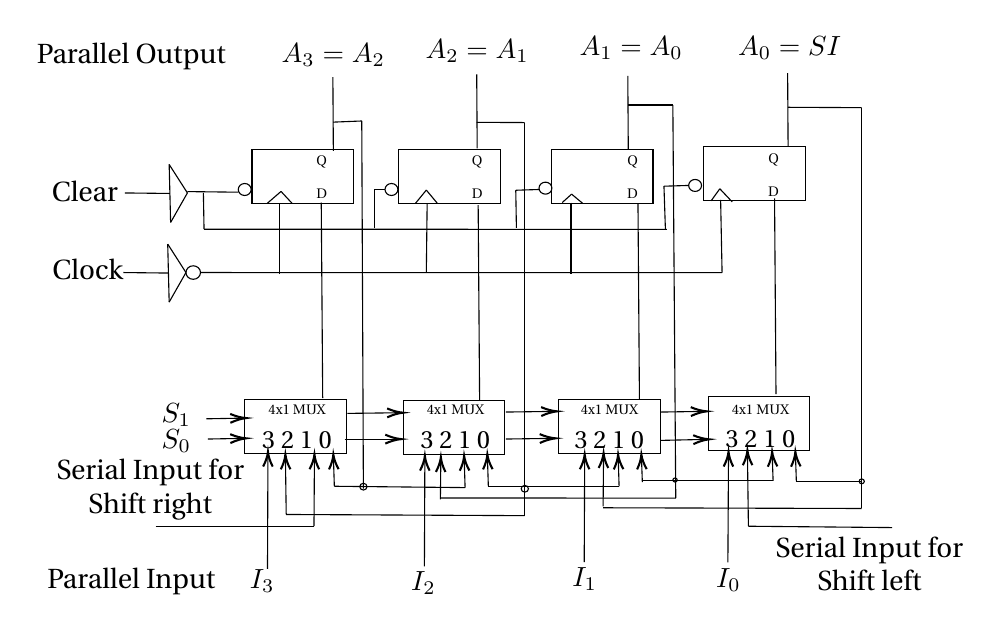
\begin{tikzpicture}[x=0.75pt,y=0.75pt,yscale=-.65,xscale=.7]
   \centering
%uncomment if require: \path (0,482.89410400390625); %set diagram left start at 0, and has height of 482.89410400390625

\draw    (247, 274) rectangle (317, 314)   ;
\draw    (138, 273) rectangle (208, 313)   ;
\draw    (354, 273) rectangle (424, 313)   ;
\draw    (457, 271) rectangle (527, 311)   ;
\draw    (244, 88) rectangle (314, 128)   ;
\draw    (143, 88) rectangle (213, 128)   ;
\draw    (349, 88) rectangle (419, 128)   ;
\draw    (454, 86) rectangle (524, 126)   ;
\draw    (111.68,287.53) -- (137,287.04) ;
\draw [shift={(139,287)}, rotate = 538.88] [color={rgb, 255:red, 0; green, 0; blue, 0 }  ][line width=0.75]    (10.93,-3.29) .. controls (6.95,-1.4) and (3.31,-0.3) .. (0,0) .. controls (3.31,0.3) and (6.95,1.4) .. (10.93,3.29)   ;

\draw    (112.68,302.53) -- (137,302.04) ;
\draw [shift={(139,302)}, rotate = 538.8399999999999] [color={rgb, 255:red, 0; green, 0; blue, 0 }  ][line width=0.75]    (10.93,-3.29) .. controls (6.95,-1.4) and (3.31,-0.3) .. (0,0) .. controls (3.31,0.3) and (6.95,1.4) .. (10.93,3.29)   ;

\draw    (153.68,398.85) -- (153.99,314) ;
\draw [shift={(154,312)}, rotate = 450.21] [color={rgb, 255:red, 0; green, 0; blue, 0 }  ][line width=0.75]    (10.93,-3.29) .. controls (6.95,-1.4) and (3.31,-0.3) .. (0,0) .. controls (3.31,0.3) and (6.95,1.4) .. (10.93,3.29)   ;

\draw    (261.68,396.85) -- (261.99,317) ;
\draw [shift={(262,315)}, rotate = 450.22] [color={rgb, 255:red, 0; green, 0; blue, 0 }  ][line width=0.75]    (10.93,-3.29) .. controls (6.95,-1.4) and (3.31,-0.3) .. (0,0) .. controls (3.31,0.3) and (6.95,1.4) .. (10.93,3.29)   ;

\draw    (371.68,393.85) -- (371.99,316) ;
\draw [shift={(372,314)}, rotate = 450.23] [color={rgb, 255:red, 0; green, 0; blue, 0 }  ][line width=0.75]    (10.93,-3.29) .. controls (6.95,-1.4) and (3.31,-0.3) .. (0,0) .. controls (3.31,0.3) and (6.95,1.4) .. (10.93,3.29)   ;

\draw    (470.56,393.89) -- (470.99,314) ;
\draw [shift={(471,312)}, rotate = 450.31] [color={rgb, 255:red, 0; green, 0; blue, 0 }  ][line width=0.75]    (10.93,-3.29) .. controls (6.95,-1.4) and (3.31,-0.3) .. (0,0) .. controls (3.31,0.3) and (6.95,1.4) .. (10.93,3.29)   ;

\draw    (185.68,367.16) -- (185.99,316) ;
\draw [shift={(186,314)}, rotate = 450.34] [color={rgb, 255:red, 0; green, 0; blue, 0 }  ][line width=0.75]    (10.93,-3.29) .. controls (6.95,-1.4) and (3.31,-0.3) .. (0,0) .. controls (3.31,0.3) and (6.95,1.4) .. (10.93,3.29)   ;

\draw    (76.68,367.16) -- (185.68,367.16) ;


\draw    (484.68,367.16) -- (484.02,313) ;
\draw [shift={(484,311)}, rotate = 449.3] [color={rgb, 255:red, 0; green, 0; blue, 0 }  ][line width=0.75]    (10.93,-3.29) .. controls (6.95,-1.4) and (3.31,-0.3) .. (0,0) .. controls (3.31,0.3) and (6.95,1.4) .. (10.93,3.29)   ;

\draw    (484.68,367.16) -- (583.68,368.16) ;


\draw    (511.68,31.27) -- (512,86) ;


\draw    (401.68,33.27) -- (402,88) ;


\draw    (297.68,32.27) -- (298,87) ;


\draw    (198.68,34.27) -- (199,89) ;


\draw    (562.68,56.9) -- (562.68,333.9) ;


\draw    (517.68,333.9) -- (562.68,333.9) ;


\draw    (511.84,56.63) -- (562.68,56.9) ;


\draw    (517.68,333.9) -- (517.06,314) ;
\draw [shift={(517,312)}, rotate = 448.21] [color={rgb, 255:red, 0; green, 0; blue, 0 }  ][line width=0.75]    (10.93,-3.29) .. controls (6.95,-1.4) and (3.31,-0.3) .. (0,0) .. controls (3.31,0.3) and (6.95,1.4) .. (10.93,3.29)   ;

\draw    (501.68,333.53) -- (501.06,314) ;
\draw [shift={(501,312)}, rotate = 448.18] [color={rgb, 255:red, 0; green, 0; blue, 0 }  ][line width=0.75]    (10.93,-3.29) .. controls (6.95,-1.4) and (3.31,-0.3) .. (0,0) .. controls (3.31,0.3) and (6.95,1.4) .. (10.93,3.29)   ;

\draw    (411.68,334.53) -- (411.07,316) ;
\draw [shift={(411,314)}, rotate = 448.09] [color={rgb, 255:red, 0; green, 0; blue, 0 }  ][line width=0.75]    (10.93,-3.29) .. controls (6.95,-1.4) and (3.31,-0.3) .. (0,0) .. controls (3.31,0.3) and (6.95,1.4) .. (10.93,3.29)   ;

\draw    (411.68,333.53) -- (501.68,333.53) ;


\draw    (562.68,354.01) -- (562.68,333.9) ;


\draw    (384.68,352.48) -- (384.98,315) ;
\draw [shift={(385,313)}, rotate = 450.46] [color={rgb, 255:red, 0; green, 0; blue, 0 }  ][line width=0.75]    (10.93,-3.29) .. controls (6.95,-1.4) and (3.31,-0.3) .. (0,0) .. controls (3.31,0.3) and (6.95,1.4) .. (10.93,3.29)   ;

\draw    (384.68,353.48) -- (562.68,354.01) ;


\draw    (305.68,337.53) -- (395.68,337.53) ;


\draw    (395.68,337.53) -- (395.06,316) ;
\draw [shift={(395,314)}, rotate = 448.33] [color={rgb, 255:red, 0; green, 0; blue, 0 }  ][line width=0.75]    (10.93,-3.29) .. controls (6.95,-1.4) and (3.31,-0.3) .. (0,0) .. controls (3.31,0.3) and (6.95,1.4) .. (10.93,3.29)   ;

\draw    (305.68,337.53) -- (305.06,316) ;
\draw [shift={(305,314)}, rotate = 448.33] [color={rgb, 255:red, 0; green, 0; blue, 0 }  ][line width=0.75]    (10.93,-3.29) .. controls (6.95,-1.4) and (3.31,-0.3) .. (0,0) .. controls (3.31,0.3) and (6.95,1.4) .. (10.93,3.29)   ;

\draw    (289.68,338.53) -- (289.06,317) ;
\draw [shift={(289,315)}, rotate = 448.33] [color={rgb, 255:red, 0; green, 0; blue, 0 }  ][line width=0.75]    (10.93,-3.29) .. controls (6.95,-1.4) and (3.31,-0.3) .. (0,0) .. controls (3.31,0.3) and (6.95,1.4) .. (10.93,3.29)   ;

\draw    (199.68,337.53) -- (199.06,316) ;
\draw [shift={(199,314)}, rotate = 448.33] [color={rgb, 255:red, 0; green, 0; blue, 0 }  ][line width=0.75]    (10.93,-3.29) .. controls (6.95,-1.4) and (3.31,-0.3) .. (0,0) .. controls (3.31,0.3) and (6.95,1.4) .. (10.93,3.29)   ;

\draw    (199.68,337.53) -- (289.68,338.53) ;


\draw    (502.68,124.22) -- (503.68,269.22) ;


\draw    (408.68,128.22) -- (409.68,273.22) ;


\draw    (298.68,129.22) -- (299.68,274.22) ;


\draw    (190.68,127.22) -- (191.68,272.22) ;


\draw    (206.68,302.59) -- (243.68,302.59) ;
\draw [shift={(245.68,302.59)}, rotate = 180] [color={rgb, 255:red, 0; green, 0; blue, 0 }  ][line width=0.75]    (10.93,-3.29) .. controls (6.95,-1.4) and (3.31,-0.3) .. (0,0) .. controls (3.31,0.3) and (6.95,1.4) .. (10.93,3.29)   ;

\draw    (317.68,302.53) -- (350,302.03) ;
\draw [shift={(352,302)}, rotate = 539.11] [color={rgb, 255:red, 0; green, 0; blue, 0 }  ][line width=0.75]    (10.93,-3.29) .. controls (6.95,-1.4) and (3.31,-0.3) .. (0,0) .. controls (3.31,0.3) and (6.95,1.4) .. (10.93,3.29)   ;

\draw    (424.68,303.53) -- (455.68,302.79) ;
\draw [shift={(457.68,302.74)}, rotate = 538.63] [color={rgb, 255:red, 0; green, 0; blue, 0 }  ][line width=0.75]    (10.93,-3.29) .. controls (6.95,-1.4) and (3.31,-0.3) .. (0,0) .. controls (3.31,0.3) and (6.95,1.4) .. (10.93,3.29)   ;

\draw    (208.68,283.53) -- (245,283.03) ;
\draw [shift={(247,283)}, rotate = 539.2] [color={rgb, 255:red, 0; green, 0; blue, 0 }  ][line width=0.75]    (10.93,-3.29) .. controls (6.95,-1.4) and (3.31,-0.3) .. (0,0) .. controls (3.31,0.3) and (6.95,1.4) .. (10.93,3.29)   ;

\draw    (317.68,282.53) -- (351,282.03) ;
\draw [shift={(353,282)}, rotate = 539.14] [color={rgb, 255:red, 0; green, 0; blue, 0 }  ][line width=0.75]    (10.93,-3.29) .. controls (6.95,-1.4) and (3.31,-0.3) .. (0,0) .. controls (3.31,0.3) and (6.95,1.4) .. (10.93,3.29)   ;

\draw    (424.68,282.53) -- (454,282.03) ;
\draw [shift={(456,282)}, rotate = 539.03] [color={rgb, 255:red, 0; green, 0; blue, 0 }  ][line width=0.75]    (10.93,-3.29) .. controls (6.95,-1.4) and (3.31,-0.3) .. (0,0) .. controls (3.31,0.3) and (6.95,1.4) .. (10.93,3.29)   ;

\draw    (272.68,347.22) -- (272.98,318) ;
\draw [shift={(273,316)}, rotate = 450.58] [color={rgb, 255:red, 0; green, 0; blue, 0 }  ][line width=0.75]    (10.93,-3.29) .. controls (6.95,-1.4) and (3.31,-0.3) .. (0,0) .. controls (3.31,0.3) and (6.95,1.4) .. (10.93,3.29)   ;

\draw    (434.68,346.32) -- (272.68,346.22) ;


\draw    (432.68,54.95) -- (434.68,346.32) ;


\draw    (401.68,54.95) -- (432.68,54.95) ;


\draw    (562.68, 333.9) circle [x radius= 1.8, y radius= 1.8]  ;
\draw    (434.18, 332.9) circle [x radius= 1.5, y radius= 1.5]  ;
\draw    (330.68,67.95) -- (330.68,359.32) ;


\draw    (166.56,358.45) -- (166.02,316) ;
\draw [shift={(166,314)}, rotate = 449.28] [color={rgb, 255:red, 0; green, 0; blue, 0 }  ][line width=0.75]    (10.93,-3.29) .. controls (6.95,-1.4) and (3.31,-0.3) .. (0,0) .. controls (3.31,0.3) and (6.95,1.4) .. (10.93,3.29)   ;

\draw    (166.56,358.45) -- (330.68,359.32) ;


\draw    (330.79, 339.39) circle [x radius= 2.5, y radius= 2.5]  ;
\draw    (297.56,67.78) -- (330.68,67.95) ;


\draw    (218.56,66.78) -- (219.68,339.32) ;


\draw    (198.84,67.63) -- (218.56,66.78) ;


\draw    (219.68, 337.84) circle [x radius= 2.5, y radius= 2.5]  ;
\draw    (55.56,120.12) -- (86.5,120.5) ;


\draw    (86,99) -- (98.56,120.12) ;


\draw    (87,142) -- (98.56,120.12) ;


\draw    (86,99) -- (87,142) ;


\draw    (138, 117.56) circle [x radius= 4.44, y radius= 4.44]  ;
\draw    (239, 117.56) circle [x radius= 4.44, y radius= 4.44]  ;
\draw    (345, 116.56) circle [x radius= 4.44, y radius= 4.44]  ;
\draw    (448, 114.56) circle [x radius= 4.44, y radius= 4.44]  ;
\draw    (98.56,119.12) -- (133.56,119.56) ;


\draw    (110,147) -- (428.56,147.12) ;


\draw    (110,147) -- (109.56,120.12) ;


\draw    (227.56,117.56) -- (227.56,146.12) ;


\draw    (227.56,117.56) -- (234.56,117.56) ;


\draw    (325,146) -- (324.56,118.12) ;


\draw    (324.56,118.12) -- (340.56,117.56) ;


\draw    (427.56,147.12) -- (426.56,115.12) ;


\draw    (426.56,115.12) -- (443.56,114.56) ;


\draw    (54.56,179.12) -- (85.5,179.5) ;


\draw    (85,158) -- (97.56,179.12) ;


\draw    (86,201) -- (97.56,179.12) ;


\draw    (85,158) -- (86,201) ;


\draw    (107.56,179.12) -- (466.56,179.23) ;


\draw    (102.56, 179.12) circle [x radius= 5, y radius= 5]  ;
\draw    (465.56,125.23) -- (466.56,179.23) ;


\draw    (362.56,127.23) -- (362.56,180.23) ;


\draw    (263.56,128.23) -- (263,179) ;


\draw    (162,128) -- (162,180) ;


\draw    (163,119) -- (170.56,127.78) ;


\draw    (163,119) -- (153.56,127.78) ;


\draw    (263,118) -- (270.56,127.78) ;


\draw    (263,118) -- (255.56,127.78) ;


\draw    (363,121) -- (370.56,127.78) ;


\draw    (363,121) -- (356.56,127.23) ;


\draw    (465,117) -- (473.56,126.78) ;


\draw    (465,117) -- (459,126) ;



\draw (150,408) node  [align=center] {$I_3$};
\draw (261,409) node  [align=center] {$I_2$};
\draw (372,406) node [align=center]{$I_1$};
\draw (471,407) node [align=center] {$I_0$};
\draw (73,340) node  [align=center] {Serial Input for\\Shift right};
\draw (568,395) node  [align=center] {Serial Input for\\Shift left};
\draw (91,285) node  [align=center] {$S_1$};
\draw (91,304) node [align=center] {$S_0$};
\draw (199,18) node  [align=center] {$A_3=A_2$};
\draw (298,15) node  [align=center] {$A_2=A_1$};
\draw (404,13) node  [align=center] {$A_1=A_0$};
\draw (513,13) node  [align=center] {$A_0=SI$};
\draw (60,408) node  [align=center] {Parallel Input};
\draw (60,19) node  [align=center] {Parallel Output};
\draw (28,119) node  [align=center] {Clear};
\draw (30,177) node  [align=center] {Clock};
\draw (191,108.5) node  [align=center] {\tiny Q\\\tiny D};
\draw (298,108.5) node  [align=center] {\tiny Q\\\tiny D};
\draw (405,108.5) node  [align=center] {\tiny Q\\\tiny D};
\draw (502,107) node  [align=center] {\tiny Q\\\tiny D};
\draw (174,293.5) node [align=center] {\tiny 4x1 MUX\\\small 3 2 1 0};
\draw (283,293.5) node  [align=center] {\tiny 4x1 MUX\\\small 3 2 1 0};
\draw (389,293.5) node  [align=center] {\tiny 4x1 MUX\\\small 3 2 1 0};
\draw (493,293) node  [align=center] {\tiny 4x1 MUX\\\small 3 2 1 0};


\end{tikzpicture}
\end{frame}
\begin{frame}
\frametitle{Parallel Load in Universal Shift Register}
When $S_0=1$ and $S_1=1$,data will be loaded from parallel input.
\tikzset{every picture/.style={line width=0.75pt}} %set default line width to 0.75pt        

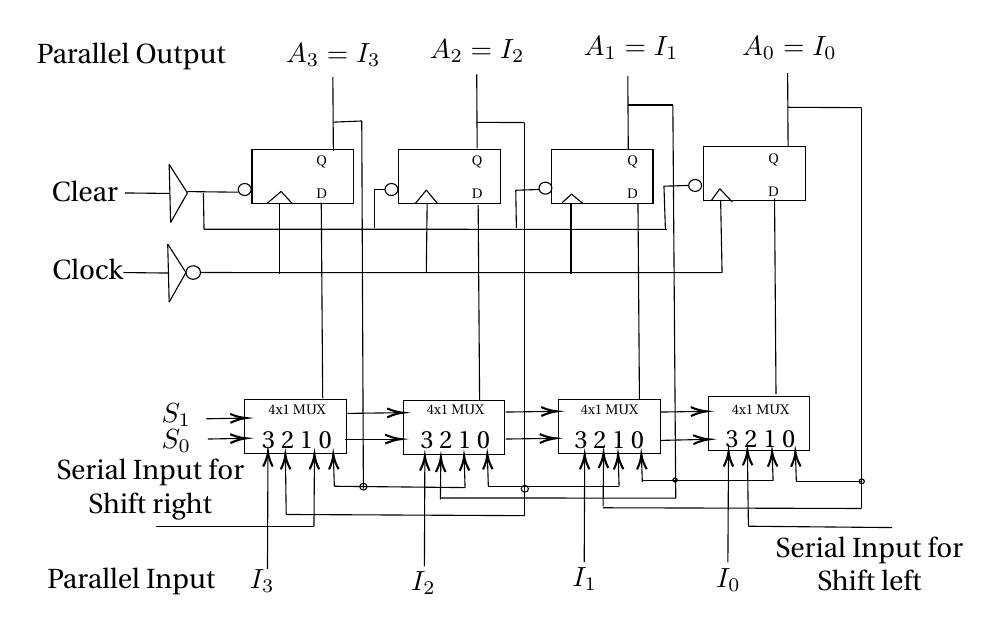
\begin{tikzpicture}[x=0.75pt,y=0.75pt,yscale=-.65,xscale=.7]
   \centering
%uncomment if require: \path (0,482.89410400390625); %set diagram left start at 0, and has height of 482.89410400390625

\draw    (247, 274) rectangle (317, 314)   ;
\draw    (138, 273) rectangle (208, 313)   ;
\draw    (354, 273) rectangle (424, 313)   ;
\draw    (457, 271) rectangle (527, 311)   ;
\draw    (244, 88) rectangle (314, 128)   ;
\draw    (143, 88) rectangle (213, 128)   ;
\draw    (349, 88) rectangle (419, 128)   ;
\draw    (454, 86) rectangle (524, 126)   ;
\draw    (111.68,287.53) -- (137,287.04) ;
\draw [shift={(139,287)}, rotate = 538.88] [color={rgb, 255:red, 0; green, 0; blue, 0 }  ][line width=0.75]    (10.93,-3.29) .. controls (6.95,-1.4) and (3.31,-0.3) .. (0,0) .. controls (3.31,0.3) and (6.95,1.4) .. (10.93,3.29)   ;

\draw    (112.68,302.53) -- (137,302.04) ;
\draw [shift={(139,302)}, rotate = 538.8399999999999] [color={rgb, 255:red, 0; green, 0; blue, 0 }  ][line width=0.75]    (10.93,-3.29) .. controls (6.95,-1.4) and (3.31,-0.3) .. (0,0) .. controls (3.31,0.3) and (6.95,1.4) .. (10.93,3.29)   ;

\draw    (153.68,398.85) -- (153.99,314) ;
\draw [shift={(154,312)}, rotate = 450.21] [color={rgb, 255:red, 0; green, 0; blue, 0 }  ][line width=0.75]    (10.93,-3.29) .. controls (6.95,-1.4) and (3.31,-0.3) .. (0,0) .. controls (3.31,0.3) and (6.95,1.4) .. (10.93,3.29)   ;

\draw    (261.68,396.85) -- (261.99,317) ;
\draw [shift={(262,315)}, rotate = 450.22] [color={rgb, 255:red, 0; green, 0; blue, 0 }  ][line width=0.75]    (10.93,-3.29) .. controls (6.95,-1.4) and (3.31,-0.3) .. (0,0) .. controls (3.31,0.3) and (6.95,1.4) .. (10.93,3.29)   ;

\draw    (371.68,393.85) -- (371.99,316) ;
\draw [shift={(372,314)}, rotate = 450.23] [color={rgb, 255:red, 0; green, 0; blue, 0 }  ][line width=0.75]    (10.93,-3.29) .. controls (6.95,-1.4) and (3.31,-0.3) .. (0,0) .. controls (3.31,0.3) and (6.95,1.4) .. (10.93,3.29)   ;

\draw    (470.56,393.89) -- (470.99,314) ;
\draw [shift={(471,312)}, rotate = 450.31] [color={rgb, 255:red, 0; green, 0; blue, 0 }  ][line width=0.75]    (10.93,-3.29) .. controls (6.95,-1.4) and (3.31,-0.3) .. (0,0) .. controls (3.31,0.3) and (6.95,1.4) .. (10.93,3.29)   ;

\draw    (185.68,367.16) -- (185.99,316) ;
\draw [shift={(186,314)}, rotate = 450.34] [color={rgb, 255:red, 0; green, 0; blue, 0 }  ][line width=0.75]    (10.93,-3.29) .. controls (6.95,-1.4) and (3.31,-0.3) .. (0,0) .. controls (3.31,0.3) and (6.95,1.4) .. (10.93,3.29)   ;

\draw    (76.68,367.16) -- (185.68,367.16) ;


\draw    (484.68,367.16) -- (484.02,313) ;
\draw [shift={(484,311)}, rotate = 449.3] [color={rgb, 255:red, 0; green, 0; blue, 0 }  ][line width=0.75]    (10.93,-3.29) .. controls (6.95,-1.4) and (3.31,-0.3) .. (0,0) .. controls (3.31,0.3) and (6.95,1.4) .. (10.93,3.29)   ;

\draw    (484.68,367.16) -- (583.68,368.16) ;


\draw    (511.68,31.27) -- (512,86) ;


\draw    (401.68,33.27) -- (402,88) ;


\draw    (297.68,32.27) -- (298,87) ;


\draw    (198.68,34.27) -- (199,89) ;


\draw    (562.68,56.9) -- (562.68,333.9) ;


\draw    (517.68,333.9) -- (562.68,333.9) ;


\draw    (511.84,56.63) -- (562.68,56.9) ;


\draw    (517.68,333.9) -- (517.06,314) ;
\draw [shift={(517,312)}, rotate = 448.21] [color={rgb, 255:red, 0; green, 0; blue, 0 }  ][line width=0.75]    (10.93,-3.29) .. controls (6.95,-1.4) and (3.31,-0.3) .. (0,0) .. controls (3.31,0.3) and (6.95,1.4) .. (10.93,3.29)   ;

\draw    (501.68,333.53) -- (501.06,314) ;
\draw [shift={(501,312)}, rotate = 448.18] [color={rgb, 255:red, 0; green, 0; blue, 0 }  ][line width=0.75]    (10.93,-3.29) .. controls (6.95,-1.4) and (3.31,-0.3) .. (0,0) .. controls (3.31,0.3) and (6.95,1.4) .. (10.93,3.29)   ;

\draw    (411.68,334.53) -- (411.07,316) ;
\draw [shift={(411,314)}, rotate = 448.09] [color={rgb, 255:red, 0; green, 0; blue, 0 }  ][line width=0.75]    (10.93,-3.29) .. controls (6.95,-1.4) and (3.31,-0.3) .. (0,0) .. controls (3.31,0.3) and (6.95,1.4) .. (10.93,3.29)   ;

\draw    (411.68,333.53) -- (501.68,333.53) ;


\draw    (562.68,354.01) -- (562.68,333.9) ;


\draw    (384.68,352.48) -- (384.98,315) ;
\draw [shift={(385,313)}, rotate = 450.46] [color={rgb, 255:red, 0; green, 0; blue, 0 }  ][line width=0.75]    (10.93,-3.29) .. controls (6.95,-1.4) and (3.31,-0.3) .. (0,0) .. controls (3.31,0.3) and (6.95,1.4) .. (10.93,3.29)   ;

\draw    (384.68,353.48) -- (562.68,354.01) ;


\draw    (305.68,337.53) -- (395.68,337.53) ;


\draw    (395.68,337.53) -- (395.06,316) ;
\draw [shift={(395,314)}, rotate = 448.33] [color={rgb, 255:red, 0; green, 0; blue, 0 }  ][line width=0.75]    (10.93,-3.29) .. controls (6.95,-1.4) and (3.31,-0.3) .. (0,0) .. controls (3.31,0.3) and (6.95,1.4) .. (10.93,3.29)   ;

\draw    (305.68,337.53) -- (305.06,316) ;
\draw [shift={(305,314)}, rotate = 448.33] [color={rgb, 255:red, 0; green, 0; blue, 0 }  ][line width=0.75]    (10.93,-3.29) .. controls (6.95,-1.4) and (3.31,-0.3) .. (0,0) .. controls (3.31,0.3) and (6.95,1.4) .. (10.93,3.29)   ;

\draw    (289.68,338.53) -- (289.06,317) ;
\draw [shift={(289,315)}, rotate = 448.33] [color={rgb, 255:red, 0; green, 0; blue, 0 }  ][line width=0.75]    (10.93,-3.29) .. controls (6.95,-1.4) and (3.31,-0.3) .. (0,0) .. controls (3.31,0.3) and (6.95,1.4) .. (10.93,3.29)   ;

\draw    (199.68,337.53) -- (199.06,316) ;
\draw [shift={(199,314)}, rotate = 448.33] [color={rgb, 255:red, 0; green, 0; blue, 0 }  ][line width=0.75]    (10.93,-3.29) .. controls (6.95,-1.4) and (3.31,-0.3) .. (0,0) .. controls (3.31,0.3) and (6.95,1.4) .. (10.93,3.29)   ;

\draw    (199.68,337.53) -- (289.68,338.53) ;


\draw    (502.68,124.22) -- (503.68,269.22) ;


\draw    (408.68,128.22) -- (409.68,273.22) ;


\draw    (298.68,129.22) -- (299.68,274.22) ;


\draw    (190.68,127.22) -- (191.68,272.22) ;


\draw    (206.68,302.59) -- (243.68,302.59) ;
\draw [shift={(245.68,302.59)}, rotate = 180] [color={rgb, 255:red, 0; green, 0; blue, 0 }  ][line width=0.75]    (10.93,-3.29) .. controls (6.95,-1.4) and (3.31,-0.3) .. (0,0) .. controls (3.31,0.3) and (6.95,1.4) .. (10.93,3.29)   ;

\draw    (317.68,302.53) -- (350,302.03) ;
\draw [shift={(352,302)}, rotate = 539.11] [color={rgb, 255:red, 0; green, 0; blue, 0 }  ][line width=0.75]    (10.93,-3.29) .. controls (6.95,-1.4) and (3.31,-0.3) .. (0,0) .. controls (3.31,0.3) and (6.95,1.4) .. (10.93,3.29)   ;

\draw    (424.68,303.53) -- (455.68,302.79) ;
\draw [shift={(457.68,302.74)}, rotate = 538.63] [color={rgb, 255:red, 0; green, 0; blue, 0 }  ][line width=0.75]    (10.93,-3.29) .. controls (6.95,-1.4) and (3.31,-0.3) .. (0,0) .. controls (3.31,0.3) and (6.95,1.4) .. (10.93,3.29)   ;

\draw    (208.68,283.53) -- (245,283.03) ;
\draw [shift={(247,283)}, rotate = 539.2] [color={rgb, 255:red, 0; green, 0; blue, 0 }  ][line width=0.75]    (10.93,-3.29) .. controls (6.95,-1.4) and (3.31,-0.3) .. (0,0) .. controls (3.31,0.3) and (6.95,1.4) .. (10.93,3.29)   ;

\draw    (317.68,282.53) -- (351,282.03) ;
\draw [shift={(353,282)}, rotate = 539.14] [color={rgb, 255:red, 0; green, 0; blue, 0 }  ][line width=0.75]    (10.93,-3.29) .. controls (6.95,-1.4) and (3.31,-0.3) .. (0,0) .. controls (3.31,0.3) and (6.95,1.4) .. (10.93,3.29)   ;

\draw    (424.68,282.53) -- (454,282.03) ;
\draw [shift={(456,282)}, rotate = 539.03] [color={rgb, 255:red, 0; green, 0; blue, 0 }  ][line width=0.75]    (10.93,-3.29) .. controls (6.95,-1.4) and (3.31,-0.3) .. (0,0) .. controls (3.31,0.3) and (6.95,1.4) .. (10.93,3.29)   ;

\draw    (272.68,347.22) -- (272.98,318) ;
\draw [shift={(273,316)}, rotate = 450.58] [color={rgb, 255:red, 0; green, 0; blue, 0 }  ][line width=0.75]    (10.93,-3.29) .. controls (6.95,-1.4) and (3.31,-0.3) .. (0,0) .. controls (3.31,0.3) and (6.95,1.4) .. (10.93,3.29)   ;

\draw    (434.68,346.32) -- (272.68,346.22) ;


\draw    (432.68,54.95) -- (434.68,346.32) ;


\draw    (401.68,54.95) -- (432.68,54.95) ;


\draw    (562.68, 333.9) circle [x radius= 1.8, y radius= 1.8]  ;
\draw    (434.18, 332.9) circle [x radius= 1.5, y radius= 1.5]  ;
\draw    (330.68,67.95) -- (330.68,359.32) ;


\draw    (166.56,358.45) -- (166.02,316) ;
\draw [shift={(166,314)}, rotate = 449.28] [color={rgb, 255:red, 0; green, 0; blue, 0 }  ][line width=0.75]    (10.93,-3.29) .. controls (6.95,-1.4) and (3.31,-0.3) .. (0,0) .. controls (3.31,0.3) and (6.95,1.4) .. (10.93,3.29)   ;

\draw    (166.56,358.45) -- (330.68,359.32) ;


\draw    (330.79, 339.39) circle [x radius= 2.5, y radius= 2.5]  ;
\draw    (297.56,67.78) -- (330.68,67.95) ;


\draw    (218.56,66.78) -- (219.68,339.32) ;


\draw    (198.84,67.63) -- (218.56,66.78) ;


\draw    (219.68, 337.84) circle [x radius= 2.5, y radius= 2.5]  ;
\draw    (55.56,120.12) -- (86.5,120.5) ;


\draw    (86,99) -- (98.56,120.12) ;


\draw    (87,142) -- (98.56,120.12) ;


\draw    (86,99) -- (87,142) ;


\draw    (138, 117.56) circle [x radius= 4.44, y radius= 4.44]  ;
\draw    (239, 117.56) circle [x radius= 4.44, y radius= 4.44]  ;
\draw    (345, 116.56) circle [x radius= 4.44, y radius= 4.44]  ;
\draw    (448, 114.56) circle [x radius= 4.44, y radius= 4.44]  ;
\draw    (98.56,119.12) -- (133.56,119.56) ;


\draw    (110,147) -- (428.56,147.12) ;


\draw    (110,147) -- (109.56,120.12) ;


\draw    (227.56,117.56) -- (227.56,146.12) ;


\draw    (227.56,117.56) -- (234.56,117.56) ;


\draw    (325,146) -- (324.56,118.12) ;


\draw    (324.56,118.12) -- (340.56,117.56) ;


\draw    (427.56,147.12) -- (426.56,115.12) ;


\draw    (426.56,115.12) -- (443.56,114.56) ;


\draw    (54.56,179.12) -- (85.5,179.5) ;


\draw    (85,158) -- (97.56,179.12) ;


\draw    (86,201) -- (97.56,179.12) ;


\draw    (85,158) -- (86,201) ;


\draw    (107.56,179.12) -- (466.56,179.23) ;


\draw    (102.56, 179.12) circle [x radius= 5, y radius= 5]  ;
\draw    (465.56,125.23) -- (466.56,179.23) ;


\draw    (362.56,127.23) -- (362.56,180.23) ;


\draw    (263.56,128.23) -- (263,179) ;


\draw    (162,128) -- (162,180) ;


\draw    (163,119) -- (170.56,127.78) ;


\draw    (163,119) -- (153.56,127.78) ;


\draw    (263,118) -- (270.56,127.78) ;


\draw    (263,118) -- (255.56,127.78) ;


\draw    (363,121) -- (370.56,127.78) ;


\draw    (363,121) -- (356.56,127.23) ;


\draw    (465,117) -- (473.56,126.78) ;


\draw    (465,117) -- (459,126) ;



\draw (150,408) node  [align=center] {$I_3$};
\draw (261,409) node  [align=center] {$I_2$};
\draw (372,406) node [align=center]{$I_1$};
\draw (471,407) node [align=center] {$I_0$};
\draw (73,340) node  [align=center] {Serial Input for\\Shift right};
\draw (568,395) node  [align=center] {Serial Input for\\Shift left};
\draw (91,285) node  [align=center] {$S_1$};
\draw (91,304) node [align=center] {$S_0$};
\draw (199,18) node  [align=center] {$A_3=I_3$};
\draw (298,15) node  [align=center] {$A_2=I_2$};
\draw (404,13) node  [align=center] {$A_1=I_1$};
\draw (513,13) node  [align=center] {$A_0=I_0$};
\draw (60,408) node  [align=center] {Parallel Input};
\draw (60,19) node  [align=center] {Parallel Output};
\draw (28,119) node  [align=center] {Clear};
\draw (30,177) node  [align=center] {Clock};
\draw (191,108.5) node  [align=center] {\tiny Q\\\tiny D};
\draw (298,108.5) node  [align=center] {\tiny Q\\\tiny D};
\draw (405,108.5) node  [align=center] {\tiny Q\\\tiny D};
\draw (502,107) node  [align=center] {\tiny Q\\\tiny D};
\draw (174,293.5) node [align=center] {\tiny 4x1 MUX\\\small 3 2 1 0};
\draw (283,293.5) node  [align=center] {\tiny 4x1 MUX\\\small 3 2 1 0};
\draw (389,293.5) node  [align=center] {\tiny 4x1 MUX\\\small 3 2 1 0};
\draw (493,293) node  [align=center] {\tiny 4x1 MUX\\\small 3 2 1 0};


\end{tikzpicture}
\end{frame}

\section{Uses}

\begin{frame}
\frametitle{Purposes of Universal Shift Register}
We can use \textbf{Universal Shift Register} in different purposes : \\
\begin{itemize}
\item Temporary data storage
\item Data transfer
\item Data manipulation
\item As counters.
\end{itemize}
\end{frame}
\begin{frame}
\frametitle{Uses of Universal Shift Register}
In practical scenario , \textbf{Universal Shift Register} is used for
\begin{itemize}
\item Serial communication of micro controller unit
\item Multiplying binary numbers
\item Storing  ALU's operands, intermediate results and final results
\end{itemize}
For performing \textbf{Universal Shift Register} operations,different ICs are used.\\
Example : IC 74194 (4 bit) and 74198 (8 bit)
\begin{columns}
\column{0.5\textwidth}
\begin{figure}[h!]
    \centering
    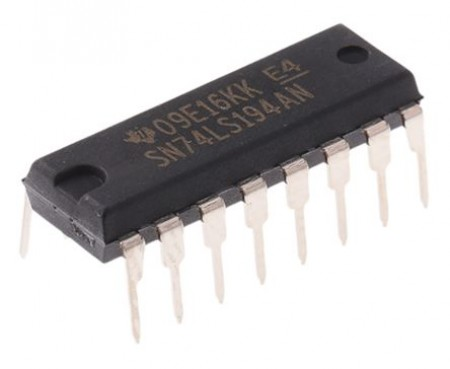
\includegraphics[width = 0.3\textwidth]{74194.jpg}
    \caption{IC 74194}
\end{figure}
\column{0.5\textwidth}
\begin{figure}[h!]
    \centering
    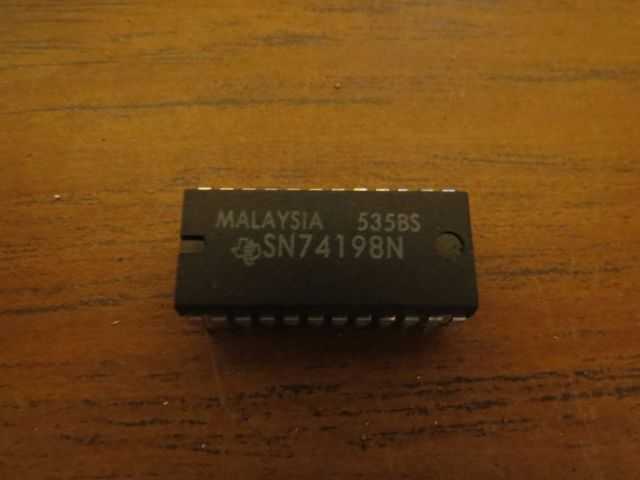
\includegraphics[width = 0.3\textwidth]{74198.jpg}
    \caption{IC 74198}
\end{figure}
\end{columns}
\end{frame}
\begin{frame}
\begin{huge}
\begin{center}

\includegraphics[width = 0.3\textwidth]{images.png}\\
Thank You!\\
Any Questions?
\end{center}

\end{huge}

\end{frame}

\end{document}